\documentclass[a4paper,11pt]{article}
\usepackage{od}
\usepackage[russian,main=english]{babel}

\author{Lebedev Yuri Valentinovich}
\title{Improving the Tools of Flow Analysis}
\date{St. Petersburg, 2015}

\setlist{noitemsep}
\newcommand{\abox}[2]{\fbox{
    \begin{minipage}[t]{#1\textwidth}\centering #2\end{minipage}
}}

\begin{document}
\maketitle

\begin{quote}
  Dissertation for TRIZ certification to the level of a TRIZ Master.

  Supervisor -- TRIZ Master S.A. Logvinov

  Translated by Hans-Gert Gräbe from the Russian Original available at
  \url{https://matriz.org/yu-lebedev/}

  Proofreading is yet required.
\end{quote}
\tableofcontents

\section{Introduction}

The work focuses on clarifying the law of improving the efficiency of flows
of substance, energy and information, and improving the methodology of flow
analysis.

In this study the flows in systems are analysed and recommendations are
formulated for increasing the practical value of the results of flow analysis
by changing the wording and conclusions of the current version of the "law of
improving the efficiency of flows of substance, energy and information" as
proposed by S. Litvin and A. Lyubomirsky. Recommendations are given to improve
the methodology and procedure of flow analysis.

\subsection{Relevance of the Research Topic}

\subsubsection{The Goals of the Study}

The purpose of this study is to improve the instrumentality of the law of flow
optimisation and to develop a practical algorithm for flow analysis.

\subsubsection{Overview of Known Approaches to this Problem}

\subsubsection*{Law of Flow Optimisation} 

The precursor of the law in question is the law of minimum energy conductivity
in systems formulated by G. Altshuller \cite{B1}. In the course of development
of the system ZRTS\footnote{Common Russian abbreviation for \emph{Laws of
    Development of Technical Systems}. -- HGG} this law for a long time (from
1975 to 2002, based on publication dates) has remained virtually unchanged. In
particular, G. Altshuller, A. Zusman, B. Zlotin mention in \cite[p. 1, 56]{B2}
the law briefly as part of the law of increasing coherence in systems;
Y. Salamatov reproduces in \cite{B3} the law almost verbatim.

The experience from practical application of the law has led to attempts to
improve it. The first work that independently analyses flows from the TRIZ
point of view is an article by Y. Khotimlyansky \cite{B4}. In V. Petrov's book
\cite{B5}, the law is considered as an increase in specific energy saturation
of systems and is a sub-trend of the law of system transition to the
microlevel.  But here it is no more considered as a requirement of a minimum
necessary level, but as a line of systems development.

Then I. Gridnev [unpublished, as reported by A. Lyubomirsky] proposed the idea
to extend this law to the whole lifetime of the system. He found that in the
process of development of a TS\footnote{Abbreviation for \emph{technical
    system}.} the conductivity of its parts carrying energy flows usually
increases, and identified mechanisms to provide this increase in conductivity.

That is why this version of the law is called \emph{Energy Conduction
  Enhancement Law}.

In the work of S. Litvin and A. Lyubomirsky \cite{B6} this approach was
extended to flows of substance and information as well.  In their system of
laws of technical development appeared a \emph{Law of increasing conductivity
  of flows of substance, energy and information} (in abbreviated form --
simply "Law of increasing conductivity of flows"). This version is the most
widespread and is the one chosen as the prototype for further work.

It is not difficult to see that with S. Litvin and A. Lyubomirsky this is
essentially a completely new law, not so much developing the predecessors as
being next to them, since:
\begin{itemize}
\item This version of the law it is not about the conditions of existence of a
  system, but about ways to improve an already viable system.
\item The range of flows to be considered is considerably extended from energy
  to all types of flows existing in the system.
\end{itemize}
The description of the law in \cite{B6} contains not only a definition of the
law itself (as trend), but also a list of sub-trends (lines of development).
They are essentially a set of recommendations to improve flows in the system.
The list of sub-trends is quite extensive and consists of 42 items. They are
structured according to the type of flow and the division of mechanisms into
"changes in the conductivity of flows" and "changes in the efficiency of
flows".

\subsubsection*{Flow Analysis}

Flow analysis has emerged and become widespread as a tool to complement the
weaknesses of Functional Analysis (FA). FA appeared in TRIZ as a tool for
finding the 'right' disadvantages \cite{B7,B8}. However, in addition to FA
itself, the so-called "functional approach" has also quickly entered the scene
and produced (and continues to produce) highly effective tools.

The reasons for this are clear. In contrast to the traditional componentwise
approach in engineering practice, the functional approach allows
\begin{itemize}
\item to consider the task from a different perspective, i.e. to remove the
  blockage of psychological inertia,
\item to abstract for a while from the design of specific components and focus
  on the functions they perform.
\end{itemize}
In FA the system is described in the form of a graph whose nodes are the
components of the system (whose structure is not disclosed), and the links are
the functions performed by the components. Here the links of the graph turn
out to be elementary machines described in terms of "object -- function --
subject". While seeming oversimplified, the approach is so productive that,
for example, it has become one of the key elements in the GEN3:ID methodology.

\textbf{Flows in a technical system are specific components. The main feature
  of a flow as component are the distributed (in space and time) parameters.}
The other components of the system (stationary) are localised in space.
Because of this distinction, flows are extremely inconvenient to fit into a
functional approach. Therefore, a special tool -- Flow Analysis
(PA\footnote{We use this Russian abbreviation to distinguish it from FA --
  Functional Analysis.}) -- has emerged.

A basic viable PA algorithm is described in \cite{B9}. Although only published
in 2010, the flow analysis methodology described therein has been effectively
applied in the company GEN3/Algorithm since at least 2003. Regardless of the
quite decent effectiveness of the methodology, specialists of GEN3/Algorithm
have made several attempts to improve it. In 2008, A. Efimov showed the
possibility of combining PA and FA in the analysis of processes \cite{B10}. In
2009, A. Kashkarov presented in his dissertation a variant of combining flow
and functional analysis \cite{B11}. In 2010, V. Vasiliev in his unpublished
work \emph{Methodology of Design of Energy Flow Chains in Mechanical TS}
considered sequences of flow transformations in a system.

\subsubsection*{Problems and Shortcomings of Existing Methodologies}

In general, the combined use of FA and PA has consistently produced good
results. However, experience from their practical application suggests to
formulate a number of problems and shortcomings. At the level of PA itself,
these are:
\begin{itemize}
\item Lack of a coherent flow parameterisation algorithm (analysed in detail
  later in the text).
\item Lack of specific recommendations to select one of the 42 available
  sub-trends.
\item Difficulty in correctly separating harmful and parasitic flows in the
  system.
\item Incorrect application of the concept of "flow conductivity" (analysed in
  detail later in the text).
\end{itemize}
At the level of interaction between FA and PA:
\begin{itemize}
\item Lack of an clear link between the elements of the functional and
  the flow model, making it difficult to formulate key deficiencies.
\item Missing relationship between the parameters of the elements of FM and of
  flows, which makes it difficult to formulate requirements for the parameters
  of the elements.
\end{itemize}
In addition, the basic papers almost completely separate the procedures for
designing a flow model and analysing this model. Thus, in O. Gerasimov's paper
\cite{B9}, after a detailed description of building the model, it is continued 
"Carry out flow model analysis", followed by literally a few lines reflecting
the main headings of the relevant chapter from the work of S. Litvin and
A. Lyubomirsky.

In the work of S. Litvin and A. Lyubomirsky \cite{B6} it is stated
\begin{quote}
  \begin{itemize}
  \item Select flows and their links related to significant disadvantages.
  \item Select the mechanisms of the law that make sense to be applied to
    address the deficiencies.
  \item Selection criteria: results of the previous analysis, availability of
    resources.
  \end{itemize}
\end{quote}
No word about the method of design of the analysed model, i.e. the selection
of the flows to be analysed.

This paper combines these two parts: model building and model analysis.

\subsection{A Detailed Statement of the Problem}

In order to improve the instrumentality of the use of the law of flow
optimisation and flow analysis, it is necessary to clarify some concepts and
definitions related to flows in systems, clarify some formulations of the law
and, in this regard, propose new methodological recommendations based on the
these formulations and concepts.

\subsection{Methods of Solving the Posed Problem}

The main methods of solving the problem were
\begin{itemize}
\item a synthesis of experiences with flow and functional analysis and ZRTS
  analysis (in the format of GEN3/Algorithm),
\item the method of classifying objects and concepts.
\end{itemize}

\subsection{The Results of the Investigations Carried Out}

\subsubsection{The results of the study are:}
\begin{itemize}
\item Introduction to a conceptual framework of flow analysis of stationary
  components which are related to flows.
\item Appropriate clarification of the provisions and wording of the law of
  flow optimisation.
\item Identifying and describing the relationship between flow and functional
  analysis, considering flow analysis as a special case of functional
  analysis.
\item Classification of flows by type.
\item Refinement of techniques and recommendations for improving flows in
  systems, taking into account their classification.
\item Three options for conducting a flow analysis are proposed, with
  recommendations of situations in which one or the other option should be
  used.
\end{itemize}

\subsubsection{Practical Relevance of the Study}

The use of the results provides an opportunity to improve the effectiveness of
the analysis, including
\begin{itemize}
\item the identification of new challenges that are not identified by FA or PA
  applied separately,
\item the clarification of flow-related tasks by locating the tasks more
  precisely.
\end{itemize}
In addition, the methodology allows to simplifies the search for directions to
solve flow problems by classifying flows in more detail.

\subsection{Key Points of the Defense}

As methodical basis for the design of flow models a functional approach in
parametric form is chosen, which is basic in the GEN3:ID methodology. And,
accordingly, functional and flow modelling used in the GEN3:ID methodology is
chosen as prototype.

The theoretical basis for the analysis of the resulting models is the ZRTS
system, also in the form of trends adopted in the GEN3:ID methodology.

The following changes have been made to the flow modelling and analysis part
of this system:

\subsubsection{Linking Flows and Other Components of the System}
\begin{itemize}
\item A definition of flow (missing so far) as a dynamic component of the
  system is introduced.
\item In accordance with this, it is proposed to consider flow analysis as a
  specific special case of functional analysis. An appropriate refinement of
  the functionally complete model of a system is proposed.
\item Based on the model of a functionally complete system, 4 types of static
  components of a functional model are distinguished, necessarily accompanying
  any flow in the system:
  \begin{itemize}
  \item Source,
  \item Channel,
  \item Receiver,
  \item Control system.
  \end{itemize}
  Similar to a functional model, each of these components (except the channel)
  may not be explicitly present or may belong to the supersystem.
\item Two main types of sources are identified and their main features are
  discussed:
  \begin{itemize}
  \item Source of a potential,
  \item Source of a stream (\foreignlanguage{russian}{ток}).
  \end{itemize}
  It is shown that consideration of these features should lead to a more
  appropriate choice of a development (improvement) strategy for the system
  containing the flows.
\item Two main types of control system are also identified:
  \begin{itemize}
  \item the type "pump",
  \item the type "valve".
  \end{itemize}
  It is shown that taking into account the type of the control system also
  enables a more deliberate choice of a strategy for improving the flow and
  the system as a whole.
\item A flow receiver is usually a working body, i.e. a key element of a
  functionally complete TS. Its analysis very often does not counts as a tasks
  of flow development, being part of an analysis of a higher system level.
  Therefore, it is not considered in this text.
\item It is shown that the flow channel is the most frequent element of flow
  improvement (along with the flow itself).
\item Based on this separation of static components associated with the flow,
  flow improvement techniques are systematised and refined, which are proposed
  in the system of trends.
\item In particular, it is shown that the reduction of conductivity of the
  harmful flow channel as recommended in the trends is an uncommon special
  case. Much more effective (and more commonly used) is a so-called "harmful
  flow channelisation", where a new channel for such a flow is formed in order
  to move the harmful flow out of the system. And the conductivity of such a
  channel must be high.
\end{itemize}

\subsubsection{Classification of Flows}
\begin{itemize}
\item As a special case of the components of a functional model, flows can be
  classified according to a number of specific characteristics. This
  classification allows for a more precise description of characteristics of
  the different flows. This makes it possible to offer additional guidance
  specific to different types of flows.
\item A classification according to the following characteristics is proposed:
  \begin{itemize}
  \item Separation of flows by functionality (useful, harmful and parasitic),
  \item Separation of flows by source (primary or secondary),
  \item Separation of flows in terms of 'horse-rider' (function or carrier),
  \item Separation of flows into closed and open flows,
  \item Separation of flows into discrete, continuous and complex.
  \end{itemize}
\item In particular, it has been proposed to distinguish between harmful and
  parasitic flows and thus offer different recommendations for them:
  \begin{itemize}
  \item Harmful flows are flows that have a harmful function (and no main
    useful function) which is predetermined by the operating principle of the
    system. For example, carbon dioxide from burning fuel in internal
    combustion engines.
  \item Parasitic flows are also flows that have a detrimental function (and
    no main useful function), but are NOT predetermined by the operating
    principle of the system. For example, nitrogen oxides and carbon monoxide
    in inadequate engine operation.
  \end{itemize}
\item For the different types and kinds of flows according to the
  classification, their typical features are described. Based on these
  features, additional techniques for their improvement are proposed.
\end{itemize}

\subsubsection{Methodology for Building a Flow Model}
\begin{itemize}
\item Two main approaches to the formulation of TRIZ analysis and working
  methods have been identified. They can be conditionally called "step-by-step
  strategy" and "step-by-step algorithm".
\item A step-by-step strategy describes the main directions, leaving enough
  room for imagination and creativity for the solver. The step-by-step
  algorithm proposes to follow literally or almost literally prescribed
  guidelines.
\item Based on the proposed combination of functional and flow analysis, two
  methodologies have been developed and tested, corresponding to a strategy
  and an algorithm and combining the benefits of both prototypes.
\item For cases where flow analysis indicates that it is appropriate to focus
  on a particular static component, a methodology has been developed and
  tested for switching from flow analysis to functional analysis.
\end{itemize}

\subsection{Personal Contribution of the Applicant}

The formulation of the research task, developing the methodology and
conducting the research, analysis of the results and the development of
methodological recommendations for flow analysis based on these results are
the personal contribution of the author.
\begin{itemize}
\item Lebedev Y.V. \foreignlanguage{russian}{Структурирование закона повышения
  эффективности использования вещества, энергии и информации} -- Structuring
  the law to increase the efficiency of substance, energy and information,
  2011.  \url{http://www.metodolog.ru/node/850}
\item Lebedev Y.V. \foreignlanguage{russian}{Классификация потоков в
  технических системах} -- Classification of flows in technical systems, 2011.
  \url{http://www.metodolog.ru/node/967}
\item Lebedev Y.V. \foreignlanguage{russian}{Метод определения несогласованных
  параметров} -- Method for determination of uncoordinated parameters, 2011.
  \url{http://www.metodolog.ru/node/992}
\item Logvinov S.A., Lebedev Y.A., Lebedev Y.V.
  \foreignlanguage{russian}{«Неразрешимые вторичные задачи».  Классификация и
    способы идентификации} -- "Intractable Secondary Problems".
  Classification and Identification Methods. TRIZ-Summit 2012.\\
  \url{http://triz-summit.ru/ru/confer/TDS-2012/205327/205392/205551/}
\item Lebedev Y.V., Logvinov S.A. Integration of flow and functional analysis.
  TRIZ-Summit 2014.  \url{http://triz-summit.ru/ru/confer/TDS-2014/article/}
\item Kuznetsova T.V., Lebedev Y.V., Logachev D.N., Logvinov S.A.
  \foreignlanguage{russian}{Особенности выполнения консультационных проектов
    на российском рынке} -- Features of Consulting Projects in the Russian
  Market, 2014.  \url{http://www.metodolog.ru/node/1780}
\item Lebedev Y.V., Logvinov S.A. \foreignlanguage{russian}{Машина Руба
  Голдберга как объект анализа} -- The Rube Goldberg Machine as an Object of
  Analysis, 2015.\\  \url{http://www.metodolog.ru/node/1910}
\end{itemize}

\section{Flows and Their Relationship to Other Components of the System}

%--Ende der Durchsicht

\textbf{A flow is the movement of material objects (matter and energy) or
  information in space in which individual moving elements move one after
  another, undergoing changes according to the same law} (part of the flow can
move in a supersystem, but the key is its presence and movement in the system
in question).

Such a definition is not exhaustive for every conceivable case, but sufficient
for practical work.

Essential to this definition is the presence of some number of elements of a
discrete flow or the possibility of dividing a coherent flow into separate
parts. A reciprocating pendulum or a rotating motor axle does not form a
flow. A car on a track does not form a flow either, although a set of cars on
a track does (and even if the set consists of a single element at a given
time).

Another important characteristic of flow is movement in space. Water flowing
in a tap or parts on a conveyor form streams. But when a tap is shut off or a
conveyor belt is stopped, the flow stops (disappears), although all the
elements of the flow remain in the system. That is, the flow is not just a set
of elements, but a set of elements movement. Therefore, \textbf{flow is a
  dynamic component of the TS}, which is its main distinguishing feature. This
is an important feature that distinguishes flow from other, "static"
components of the TS: flow can "disappear" from the system without removing
any parts from it.

\subsection{Functionally complete TS and its relation to FA}

The functional approach in TRIZ, though formulated rather late, goes back to
the very origin of TRIZ. Namely, the law of completeness of system parts
formulated by G. Altshuller as the first of the laws of technical development
[e.g., in \cite{B1}]:
\begin{quote}
  A prerequisite for the fundamental viability of a technical system is the
  availability and minimum operability of the main parts of the system. Every
  technical system must include four main parts: engine, transmission,
  operating organ and control organ.
\end{quote}

For the sake of generality, it makes sense to replace the terms engine and
transmission in this formulation with energy source and energy converter.

The general diagram of a functionally complete TC is as follows
\begin{center}
  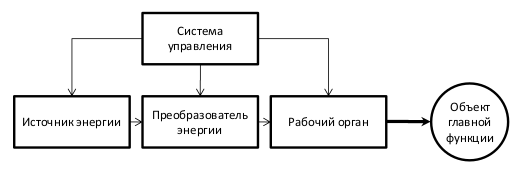
\includegraphics[width=.8\textwidth]{1.png}
\end{center}

Of course, real systems are usually more complex. This law establishes only
the minimum components required to be functional.

A Functional Model (FM) is essentially such an extended schema. It should be
understood that each function of the FM is performed by its own functionally
complete minimachine. And the component that is mapped to the FM may include
this entire machine in its composition, or it may use other components.

\subsection{Functional and complete flow subsystem}

In the case of a flow, it is not localised to a point. Therefore, a scheme of
a functionally complete minimax operating on a flow should look somewhat
different.
\begin{center}
  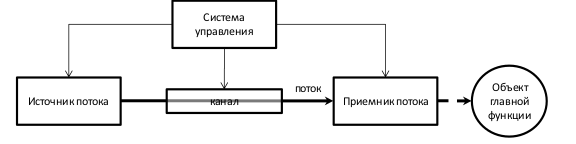
\includegraphics[width=.8\textwidth]{2.png}
\end{center}
More traditional Sankey diagrams for flow analysis (see e.g. \cite{B12})
\begin{center}
  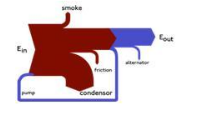
\includegraphics[width=.8\textwidth]{3.png}
\end{center}
either completely ignore the component component or, at the very least, the
functional (out-of-flow) links between components:
\begin{center}
  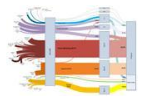
\includegraphics[width=.8\textwidth]{4.png}
\end{center}
In this paper, a flow is treated as a peculiar, but one component of a
system. Also, components of its implementation such as source, channel and
receiver are introduced into the description of the flow. Moreover, in fact,
in a real analysis this is always the case, without which the analysis becomes
no more than a pretty design.

Three important conclusions can thus be drawn:
\begin{enumerate}
\item \textbf{A flow is a component of the system and as such performs one or
  more functions. A flow function is defined in the same way as in FA, i.e. as
  the action of changing at least one parameter of the function object.}
\item \textbf{A flow in a system, similar to components in an FA, is always
  linked to a set of other components in such a way that together they form a
  virtual machine that provides the flow function.}
\item \textbf{Considering the flow with other functional (stationary)
  components allows for joint flow and functional analysis, which can markedly
  improve the quality of the analysis.}
\end{enumerate}
The first conclusion is obvious to the point of triviality. But,
unfortunately, it has not yet been properly verbalised. In particular, this is
why functional analysis and flow analysis are still performed as two
completely unrelated analyses.

The second conclusion is also clear. Moreover, in real projects, flow-related
components and their properties are always taken into account too. But they
are only considered in their relationship to the flow. But at the same time,
they are also system components and usually have functional relationships that
are considered in the FM. However, their functional relationship affects their
interaction with the flow and vice versa. A simple example: the flow in a pipe
causes corrosion of the components it washes. Hence, the "holding" function of
the pipe walls starts to be performed inadequately. When PA and FA are used
separately, this phenomenon can hardly be seen. In order to take this
circumstance into account, one has to "work out" somehow in both types of
analysis. To make it worse, the effect must be first seen and then included
into the analysis. This causes the analysis efficiency to drop drastically.
After all, the analysis is done to see the effects of functional
relationships, not just to list previously seen effects.

The third conclusion paves the way for the creation of a combined analysis
methodology. Several options for such a methodology will be proposed below.

As a matter of fact, the very original scheme of a functionally complete
machine already suggests such a possibility of unification. However, as noted
above, this scheme goes back to the very foundations of theory. This confirms
the validity of the proposed approach. Indeed:
\begin{center}
  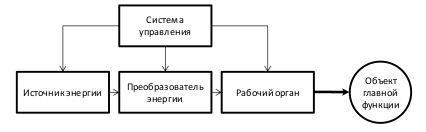
\includegraphics[width=.8\textwidth]{5.png}
\end{center}
This diagram shows almost explicitly the energy flows from the source to the
inverter and on to the actuator, and the information flows from the control
system.

In principle, it would be possible to mark both the flows and the functional
relationships directly on this diagram. But it should be understood that this
diagram is the minimum diagram of a minimally functional machine. The FM of
any real TS is always more complicated. Combining both flows and functional
connections in one model will lead to unreasonable complication and
oversaturation of the model, which will lead to its actual inoperability.

A close approach to this was suggested by A. Kashkarov in his 2009 Master
Paper \cite{B11}. It is difficult to disagree with the thesis of the paper.
But, unfortunately, the proposed technique of joint analysis is very
labour-intensive, which reduces its applicability in projects

\subsection{Flow channel as the main tool for flow management}

Most often, flow optimisation comes from channel improvement and, to a much
lesser extent, from source and consumer improvement.

This is due to the law of non-uniform development of system parts: both the
consumer and the source are the working body (not necessarily the main
one). Therefore, their development comes before the development of the channel
(transmission in Altshuller's formulation, when he talked about energy flows
in mechanical and electromechanical systems). Therefore, when the task of
optimising flows comes up in a real working project, the optimisation of work
tools has usually already been carried out and they are at the level of
development that is available for a given system here and now. The task of
improving flow sources and flow consumers (flow receptors) can be set, but
almost always as a forward-looking task.

For example, in an internal combustion engine there is a flow of contaminants
in the oil. As both a source and the "consumer" of this flow is the friction
components (closed flow case). In addition to installing filters (channel
control), it is possible to aim at reducing friction. For example, magnetic
bearings completely or almost completely eliminate friction and thus
drastically reduce contamination. But it must be understood that such a source
conversion, if done, is done for other reasons (reducing friction in moving
components is in itself a much more important task than reducing contamination
in oil). Therefore:
\begin{itemize}
\item Such work is done for other reasons and has nothing to do with
  optimising oil flow,
\item In any particular system, the existing level of friction is set either
  by technical possibilities or by economic and other constraints and is
  usually not manageable at this stage of system development.
\item Nevertheless, this \textbf{flow} control option should be kept in mind
  (although it is most often not used)
\end{itemize}
Another example. On a production line, the scrap flow is a typical parasitic
flow that must always be reduced. To improve the process, all three components
are changed:
\begin{itemize}
\item The equipment where the defect occurs (source of flow),
\item Rejects and rejects system (flow channel),
\item Equipment of the next operation (consumer).
\end{itemize}
Of course, all three need to be improved. BUT:

It is reasonable for future projects to design equipment with a lower
rejection rate (source) and a higher tolerance (consumer). In the non-TRIZ
environment, this is formulated as a requirement for equipment designers to
provide a larger range of input parameters and a smaller range of output
parameters. Some other system improvement techniques, such as DFSS, have a
similar objective. But it is reasonable to set such a goal for the equipment
manufacturer, i.e. in this case a completely different system would be
considered.

If, on the other hand, work is being done to improve a process that already
uses the specified equipment, then the equipment parameters are a supersystem
factor that is difficult to change (it makes no sense for a bread producer to
propose solutions related to the development of a new oven as well as to the
development of new wheat varieties). Therefore, in ongoing system improvement
projects, rejection management (flow channel) is often the only option
available.

\subsection{Parametric description of the flows}

The functional approach to describing systems also implies a parametric
description. That is, a description of the main parameters of the functions in
question.

Indeed, a function is an action that changes at least one parameter of an
object. But in this way, a description of a function without specifying its
parameters (the parameters of the specified action) becomes purely speculative
and results in an empty functional model, only explaining what was known in
advance. Not to mention that the refusal to parameterise leads to unworkable
ideas, which at best entails a waste of time, and at worst up to the failure
of the project.

In FM, however, a set of parameters can only be chosen for general engineering
reasons. This is simply because FM deals with a whole host of TCs, differing
in everything except perhaps the presence of the four mandatory components.

These flows are special cases of components and have certain common
characteristics. Therefore, it is possible to classify according to these
common characteristics and thus at least partially generalise the
parameterisation procedure.

\subsection{Types of sources}

Streams can be divided into two broad types according to the type of source.
\begin{itemize}
\item The source that creates the force that moves the flow. Most often it is
  a continuous (coherent) flow.
\item The source that creates (dispenses) the elements of a stream. Most often
  this is a discrete stream.
\end{itemize}
The first is, for example, an electric current (the source gives off an
electric potential difference) and water/air flow (the source creates a
pressure difference).

In the second case, it is, for example, the flow of parts on an assembly line
(the source is the previous equipment that dispenses the parts) and the
passenger flow on public transport (the source is the various kinds of rooms
from which people go out into the street).

Clearly, these two types of flows need to be described and analysed
differently.

\subsubsection{Flux from a potential difference source}

Such flows can be described by the formula
\begin{gather*}
  I = U\cdot\sigma(U) = U/R(U).
\end{gather*}
$I$ is the magnitude of the flow, measured in flow elements per unit time
(electric current in coulombs per second; air flow in cubic metres per hour,
etc.)

$U$ is the potential created by the source. I.e. -- the force with which the
source acts on the flux per unit of flux (Volt = 1 Newton per coulomb)

$\sigma$ -- The conductivity of a channel, i.e. the value that characterises
the ability of a channel to transmit flux. It is measured in the amount of
flux per unit potential.

$R$ is the flow resistance of the channel, i.e. the value that characterises
the braking of the flow by the channel.

Already from this formula three important conclusions are immediately
apparent:
\begin{enumerate}
\item The necessity (relevance) of dividing a flow-related system into flow
  itself, channel and source: "Flow force" is a characteristic of the flow
  itself, potential difference is determined by the source, resistance by the
  channel.

  Note: Strictly speaking, the potential difference between the source and the
  consumer is determined by the potential of each of them. However, it is
  usually the source that determines this value.
\item The instrumentality of the approach. It is not always easy to identify
  which parameter in a given system is potential and which is resistance
  (unless, of course, we are talking about classical, "school" cases like a
  circuit of electric current). But it must be done: it is immediately clear
  which parameter needs to be worked on.
\item Since it is necessary to ensure a given "current" when working on flow,
  it is immediately clear that this can be done in two ways. In other words,
  two significantly different areas of further improvement are immediately
  outlined: working with "potential" and working with "resistance".
\end{enumerate}

\subsubsection*{Linear and non-linear fluxes from a potential difference
  source} 

Fluxes from a potential difference source, in turn, can be divided into linear
and non-linear. That is, into one where the resistance is independent of
potential or current, and one where it is dependent.

It should be stated at the outset that there are no truly linear flows, there
is always non-linearity. But within each given problem and within a given
range of values, non-linearity can often be neglected. It is this kind of flow
that is called linear.

\textbf{The point of this division is that non-linearity means that not only
  the flow is dependent on the channel, but also the channel is dependent on
  the flow. That is, the channel in this case appears dynamised. This is the
  reason for many disadvantages. But also many opportunities.}

Linear flow lacks this capability. And it is very often desirable to introduce
such non-linearity. At the very least, it is a good additional possibility
(see dynamisation law).

As an example, suffice it to recall that the advent of non-linear elements in
electrical engineering has literally transformed the world. This is despite
the fact that the share of electricity in total energy consumption has
remained relatively modest, far below 50\% [see e.g. \cite{B13}].

\subsubsection{Element source flow}

The flow from the element source is quite different from the previous one.

Such flow is characterised by source power $W_s$ (source) and channel
bandwidth $W_c$ (channel).

The flow is described as follows:

If $W_s>W_c$, the amount of flow will be equal to $W_c$. I.e., there is as
much flow through the channel elements as much as it can pass through. But the
source output will either be jammed (traffic jam), or it will not operate at
full capacity. In other words, there is an obvious a bottle-neck situation.
But at the same time it turns out not to be described by speculative, but
numerical.

If $W_s<W_c$, the amount of flow will be equal to $W_s$. This means that as
many elements will flow through the channel as the source can deliver. But the
channel will be underloaded (half-empty trains, a nearly dried-up stream).
Here too, everything seems to be clear without any additional classification,
but the situation turns out to be parametrized.

\section{Flow types (classification)}

\subsection{Possibility and feasibility of classifying flows}

One of the main advantages of traditional functional analysis -- its
universality -- is achieved through a very high level of
generalisation. Components are treated as a kind of universal black box (with,
of course, the possibility to consider them in more detail if necessary).
Functions often tend to be generalised to a narrow set of generalised
functions. This is perfectly justified for a number of reasons, but it also
leads to certain difficulties in further analysis: the recommendations of the
methodology are forced to be generalised to no lesser level.

The recognition of a flow as a specific component of a system allows us to
apply the signs of classification to them. As a matter of fact, this fact can
already be seen in the work of Litvin and Lyubomirsky \cite{B6}, where the
primary classification of flows is made. However, it is possible to give a
substantially more detailed classification of flows without violating
generality. And, accordingly, considerably concretise the resulting
recommendations.

Litvin's and Lubomirski's work divides streams in two ways.
\begin{itemize}
\item by nature (matter, energy and information flows)
\item on the basis of functionality (useful, harmful and parasitic flows).
\end{itemize}
The first indication is unmistakable. Although the duality of many fluxes does
occasionally come up. For example, an electrical signal is a flow of electrons
electronic circuitry (matter), electrical energy or information? Usually the
question is decided according to the task at hand. If the task is interested
in the information component -- the flow is considered as a signal, if the
board is interested in heating -- as energy, if the physical principles of
operation are analysed -- as electrons (holes, ions, etc.). But in fact, there
are three different fluxes closely related to each other. And -- not
necessarily with unambiguous connection. This ambiguity of connection of three
kinds of flows opens additional possibilities for development (perfection) of
systems. Not taking this factor into account does not make the analysis
inherently wrong, but it narrows the scope for problem setting and subsequent
problem solving.

It follows from this that a more detailed classification of flows as compared
to components
\begin{itemize}
\item[B)] is possible
\item[A)] is appropriate.
\end{itemize}

\subsection{Separation of flows by functionality}

\begin{itemize}
\item \textbf{Useful streams in a system are streams intended to perform a
  useful function in the system} (regardless of the quality of performance),
\item \textbf{Harmful flows in the system are flows NOT intended but
  unavoidable} according to the operating principle or coming into the system
  from outside (external),
\item \textbf{Parasitic flows -- flows that are not required by the chosen
  operating principle} and that perform a harmful function or impair the
  performance of a useful function, arising from design imperfections.
\end{itemize}
It may seem that the mere recognition of flows as components of a system makes
it meaningless to divide them into useful and harmful components. Indeed, it
is not common in functional analysis to divide components into useful and
harmful. If a flow whose main function is harmful is called harmful, it is
clear that the designers did not introduce this flow on purpose. This flow
either arose in the process of functioning or came from a supersystem. In
principle, harmful stationary components can be formulated: components that
have arisen during the functioning of the TS or components of the supersystem
that perform harmful functions. For example, pollutants of all kinds. It is
clear that in FA the occurrence of such a component unambiguously triggers the
elimination task and therefore no additional classification is needed.

However, this is not the case with a flow. Above, a flow has been recognised
as a "virtual" component which can arise and disappear as a result of
interaction with other components. Harmful or parasitic flow can result from
component interactions (in the case of a parasitic flow, a useful but
inadequately performed interaction, in the case of a harmful flow, a harmful
interaction). In addition, a flow travels through the system and often there
may be a situation where a flow performs the useful function for which it was
created, in one place in the system, and then turns into a harmful one.
Finally, flow can enter the system from outside the system.

Thus:
\begin{itemize}
\item \textbf{Harmful flows in the system objectively exist.}
\item \textbf{The different ways in which they are formed also allow for an
  additional classification to be applied}.
\end{itemize}
Just as in FA, one can set a goal of unconditional elimination of harmful
fluxes. But harmful flow (as well as 'harmful component') is an intractable
consequence of the chosen operating principle. Therefore, a more detailed
classification of fluxes makes a lot of sense in order to choose the right way
to minimise the harmful flux or its detrimental effect.

\subsubsection{Typical techniques for optimising beneficial and minimising
  harmful flows, taking into account the main components}

Chapter 5.1.4. of \cite{B6} lists just over forty "subtrends" of flow
optimisation. In essence, this list is a fairly comprehensive list of
techniques to address the weaknesses identified in the flow analysis. These
techniques are also described in some detail and illustrated with examples. A
detailed description is not required in this paper. Some features, determined
by the identification of "stationary" components associated with the flow, as
well as the structuring of flows, will be given later in the chapters "Harmful
flows. Work with flows depending on classification" and "Useful flows.
Workflows depending on classification".

In a sense, the list is analogous to Altshuller's 40 techniques. The list is
almost completely unstructured, apart from dividing streams into useful and
harmful ones.

When stationary components are matched to each flow, it is possible to make
more precise recommendations on the application of these techniques.
\begin{center}
  \abox{.4}{The positive effect of a flow}

  \abox{.25}{Improvement of the consumer}\hfill
  \abox{.25}{Improvement of the source}\hfill
  \abox{.25}{Improvement of the channel}
  
  \abox{.3}{
    \begin{itemize}[leftmargin=10pt]
    \item Preliminary saturation of the working area
    \item Convert the receiver to a better flow sensitivity
  \end{itemize}}\hfill
  \abox{.3}{
    \begin{itemize}[leftmargin=10pt]
    \item Improve the specific characteristics of the flow or the source
    \item Flow modulation (including conversion to a pulsed flow)
    \item Giving the flow additional useful functions
    \item Use of gradients
    \item Reuse of the flow
    \item Use of an additional flow to reinforce the useful effect of the flow
    \item Use of resonance
    \item Decrease the flow intensity by switching to a self-regulating flow
  \end{itemize}}\hfill
  \abox{.3}{
    \begin{itemize}[leftmargin=10pt]
    \item Eliminating bottle necks
    \item Removes dead zones
    \item Removes grey areas
    \item Changing the flow carrier 
    \item Outsource the flow to the supersystem
    \item Reduce the number of flow transformations
    \item increasing the conductivity of the channel links
    \item Reduce channel length
    \item Put multiple useful flows in one channel
  \end{itemize}}
\newpage
  
  \abox{.4}{The negative effect of a flow}

  \abox{.25}{Improvement of the consumer}\hfill
  \abox{.25}{Improvement of the source}\hfill
  \abox{.25}{Improvement of the channel}
  
  \abox{.3}{
    \begin{itemize}[leftmargin=10pt]
    \item Pre-saturation of the working area 
    \item Convert the receiver to be less flow sensitive
    \end{itemize}}\hfill
  \abox{.3}{
    \begin{itemize}[leftmargin=10pt]
    \item Decrease specific flow characteristics 
    \item Avoid the flow
    \item Use of gradients
    \item Uniformly distribute the flow over time 
    \item Beneficial use of a harmful flow 
    \item Insertion of a second flow to correct the damage from the first flow
    \item Combine the flow with an antiflow
    \item Remove the flow by adding it with itself
    \item Remove resonance
    \end{itemize}}\hfill
  \abox{.3}{
    \begin{itemize}[leftmargin=10pt]
    \item Put the flow in a channel
    \item Installing in the path of the flow bottle necks or dead zones
    \item Reduce the conductivity of the flow channel
    \item Increase the channel length
    \end{itemize}}
\end{center}

This division is superficially similar to the division of Altshuller's 40
techniques made by ARIZ-91 (St. Petersburg) \cite{B14}, although it differs in
the genesis of the division.

A detailed description of the individual techniques is given in sufficient
detail in the work of Litvin and Lyubomirsky and requires no further
justification. At the same time, the proposed division allows:
\begin{itemize}
\item Increase the efficiency of the analytical and decision-making procedures
  by reducing the overshooting of options.
\item Focus the identified weaknesses and therefore the objectives on the
  specific components of the system under analysis
\end{itemize}
\newpage
In addition, it is possible to select (or rank) different solutions depending
on the conditions of the project:
\begin{center}
  \abox{.4}{The positive effect of a flow}

  \abox{.25}{Improvement of the consumer}\hfill
  \abox{.25}{Improvement of the source}\hfill
  \abox{.25}{Improvement of the channel}
  
  \abox{.6}{$\Longleftarrow$ The easy way (short solution) $\Longleftarrow$}

  \abox{.6}{$\Longrightarrow$ The effective way (long
    solution)$\Longrightarrow$}

\vskip2em

  \abox{.4}{The negative effect of a flow}

  \abox{.25}{Improvement of the consumer}\hfill
  \abox{.25}{Improvement of the source}\hfill
  \abox{.25}{Improvement of the channel}
  
  \abox{.6}{$\Longleftarrow$ The easy way (short solution) $\Longleftarrow$}

  \abox{.6}{$\Longrightarrow$ The effective way (long
    solution)$\Longrightarrow$}

\end{center}

This is made possible by the law of unequal development of the parts of the
system \cite{B6}, according to which the first in the system is the working
body, followed by the transmission and then the source. In this case, the flow
receptor is usually the working body (a component of a higher functional rank)
and, by virtue of the law of non-uniformity development of the parts of the
system, develops before the other components. So by the time The flow
optimisation task is often already developed to the point where which it is
possible to do in the "here and now". The source of the flow, the primary
shaping it parameters, is most often a component of a lower functional rank.
But on the other hand, it is more often a supersystem component and its
improvement may also be difficult or impractical for each given task. The
channel, on the other hand, is an auxiliary component whose only useful
function (at least in the context of flow analysis) is to direct the flow.
Therefore, its improvement can proceed painlessly for the functioning of the
system as a whole. At the same time, the channel largely determines the
efficiency of the flow.

As a result, in order to improve a system quickly, albeit in a shallow way
(which is often the case), one must first try to improve the channel, then the
source (if permitted by the design constraints) and only at the very end the
working body (the receiver). If, however, the requirements are set for
in-depth if the system is to be improved, first the possibilities of improving
the working body (up to and including changing the principle of operation)
should be analysed, and then the components that ensure its operation. As a
matter of fact, a similar recommendation exists in FA, where it is expressed
in the form of ranking the functions according to their functional importance
(see, e.g., \cite{B16}).

Parasitic flows are, by definition, flows that are \emph{not unavoidable} in
principle, but that either perform a harmful function or impair the adequate
performance of a useful function. Therefore, the first recommendation is to
eliminate such flows completely. If this fails, then the parasitic flow should
be dealt with according to the same rules as for harmful flows.

\subsection{Classification of flows according to other characteristics}

In addition to the division of flows by their nature (substance, energy,
information) and functionality (useful, harmful, parasitic), it is also
advisable to divide flows by some other characteristics. The classification
proposed in this paper is not the only possible, but it seems optimal:
distinguishing flows by these characteristics most often leads to
significantly different conclusions and recommendations:
\begin{itemize}
\item \textbf{Separation of flows by source (primary or secondary)},
\item \textbf{Separation of flows in terms of 'horse-rider' (function or
  carrier)},
\item \textbf{Separation of streams into closed and open streams},
\item \textbf{The division of flows into discrete, continuous and complex}.
\end{itemize}
See below for a more detailed description.

In situ, depending on the task at hand, other classification attributes may
also be used. Such additional characteristics may include, for example:
\begin{itemize}
\item system rank (main or auxiliary flow) -- depending on what function the
  flow performs in the system,
\item localised or distributed,
\item stationary or non-equilibrium flow,
\item easily or hardly manageable (difficult to control) flow,
\item etc. -- but this kind of classification should be introduced ad hoc.
\end{itemize}
The main flow is the flow that directly performs the main function of the
system or that provides it to the corresponding component. An auxiliary flow,
similar to an auxiliary function in FA, is defined as a flow which provides
that function to the main flow, but which has no independent significance.

A localised flow is one that flows in a channel with clearly defined
boundaries. Distributed flow is flowing in a channel with unspecified
boundaries or one for which the channel is the entire volume of the system.

A stationary flow is a flow with constant parameters over time.  A
non-equilibrium flow is a flow whose parameters change over time.

Of course, whenever there is a real analysis in a project, the industry
classification must also be taken into account: direct or alternating current
in electrical engineering, sound or ultrasound in acoustics, group or
individual processing in technology, etc.

\subsubsection{Separation of flows by source (primary or secondary)}

\textbf{The primary flow is the flow coming from the supersystem; the
  secondary flow is the flow generated within the system.}

It is clear that these flows must be handled according to different rules,
which the current version of the methodology does not take into account.

For example, a primary utility stream is often unambiguously defined by its
parameters and it is virtually impossible to modify it. In an extreme case, it
is possible to transform the flow, i.e. to form a new flow, already secondary,
from the original primary flow. It is clear that it is an extreme case as it
knowingly complicates the system. For example, compression of atmospheric air
in an internal combustion engine.

In this case, the concept of secondary useful flow refers directly to the
properties of the source. This means that even the separation of flows in this
way helps to identify immediately the component of the system to be improved.

Similarly with noxious flows. The primary detrimental flow must (preferably)
be directly inhibited at the inlet. At the same time, the secondary harmful
flow is, by definition, shaped by the operating principle and cannot be
prevented without changing the operating principle.

Thus, just a proper classification on this basis can quickly point the way
towards solutions.

\subsubsection{Dividing flows by function or medium}

Many flows in the system have the only useful function of carrying another
flow. For example, for substance flows, these are group container flows in
shop floor or transport logistics. Their only purpose is to carry some other
flow, which actually performs a useful function.

Accordingly:
\begin{itemize}
\item \textbf{A carrier stream is a stream intended (performing the function
  of) transporting some other stream.}
\item \textbf{A function stream is a stream that actually performs a function
  other than that of the carrier stream.}
\end{itemize}
A phenomenon very common when considering matter flows. Energy flows almost
always and information flows simply always require the involvement of a
carrier flow.

In the current version of the methodology, there is only one hint of such a
division:
\begin{quote}
  The use of one flow as a carrier of a second flow. A regularity in the
  development of technical systems, consisting in the transition from
  independent transmission of heterogeneous flows to the carriage of one flow
  by another \cite{B6}.
\end{quote}

But here we are talking about the possibility (and it is emphasised that
sometimes) of giving some kind of flow a carrier function, nothing more.
Meanwhile, the phenomenon is extremely widespread in technology.

The presence of a useful flow of matter in the system almost always guarantees
the existence of at least two other useful flows supplied by the carrier.

For example:

It would seem that what kind of carrier flux acts in a flat on the water that
flows from the tap? But for the water to flow, there has to be a controlling
effect, which requires a flow of information. That flow needs a carrier. And
it also needs energy to turn off the tap. This energy also has its own medium.
It is not always the case that these flows need to be considered in PA and in
the solution of a particular problem. But what is important is that they are
there. For example, the principle of medium substitutability (see below) has
been applied to the design of taps that open when hands are placed on them.

Hydrocarbon fuels are often carriers of various types of additives (and the
resulting mixture is a carrier of chemical energy)

In batch processingq, the workpieces (semi-finished products) are arranged in cassettes (boxes, trays, etc.)

Tara is a typical flow carrier.

It has already been mentioned that water is the carrier of the auxiliary flow
of salts in the preparation of all kinds of brines (and the brines themselves
are often used as carriers of the "cold" flow).

The operator's labour cost stream (a specific, but quite real auxiliary useful
stream costing the employer real money) is a typical carrier stream Useful
streams (functions) for production are streams of decisions made and actions
taken. This creates a harmful (from the employer's point of view) secondary
'labour cost' flow (not always mandatory and very often -- inadequate...).

Etc.

Thus, the separation of flows into medium and function is essential and
deserves to be analysed in its own right.

\subsubsection{Dividing flows into closed and open}
\begin{itemize}
\item \textbf{Closed threads are defined as threads that are returned to their
  source for reuse.}
\item \textbf{Open threads are either those that are discarded into the
  supersystem after use, or those that are dissipated altogether.}
\end{itemize}
The current version of the methodology \cite{B9} considers only open flows.
This approach is possible for two reasons:
\begin{itemize}
\item Closed-circuit flows are used much less frequently. Mainly found as
  carrier flows.
\item They can be regarded as open because the closed stream returns to the
  source with modified properties, requires some kind of processing to reuse
  and can therefore be regarded as two different streams with different
  parameters (before and after conversion).

  Nevertheless, closed and open streams have significantly different
  properties and can be improved by different techniques.
\end{itemize}

\subsubsection{Separation of flows by connectivity}

The flows in the system are divided into:
\begin{itemize}
\item Discrete (multi-component)
\item Bound (solid)
\item Comprehensive
\end{itemize}
The principle of separation is clear. For example, flows of parts on an
assembly line or cars on a highway are discrete flows. A flow consists of
complete units -- the elements of the flow. Any such element can be removed
from the flow and treated as an independent component of the system. The flow
is formed not so much by these elements, but by their movement according to
the same law. The simplest attribute: the units are pieces per unit of time.

A variety of liquid and gas flows are examples of continuous flows. It is
usually not possible (or practical) to isolate a single element and consider
it on its own. The static component here can be considered to be the totality
of the material being moved (in the case of a flow of matter). Characteristic:
For a static component, the unit of measure is kilograms, litres, etc.; for a
flow, it is kg/sec, litres/min, etc.

Energy flows also refer to continuous flows.

Complex flows combine features of both of the previous options.

For example, the rock flow in a rock avalanche consists of individual rocks,
each of which can also be considered as a separate component of the avalanche
-- it is a typical discrete flow. In contrast, debris flow consists of a
mixture of two or three different flows (water flow -- continuous; rock flow
-- discrete; clay slurry flow -- continuous and complex within itself).
Depending on the problem to be solved, it may be necessary to consider these
flows separately, but in science the mudflow is considered as a single complex
flow (see, for example, \cite{B18}).

Another example: the flow of information in digital form consists of
individual bytes, in textual form of words. Both bytes and words can be
treated as separate components and analysed separately. When put together,
they acquire an additional quality.

The sign of complex flow: the unit of measurement is the number of different
discrete elements.

However, in each situation, a complex flow should be considered either
discrete or continuous, depending on the problem. However, in any given
situation, a complex flow should be considered either discrete or continuous,
depending on the problem.

It is clear that discrete and continuous flows have slightly different
properties.  The main difference lies in the way it is generated, i.e. in the
source of the flow. For Continuous flows are characterised by a "source of
potential", discrete flows by "current source". The differences will be
discussed in a later chapter. After the output from the source, both types of
flow behave closely. For example, the flow of cars on a track of limited width
can be described by equations, surprisingly resembling Ohm's, Kirchhoff's and
Bernoulli's laws.

\subsection{Example of classification}

It is convenient to consider the internal combustion engine as an example of
the proposed classification.
\begin{itemize}
\item Separation of "source/channel/stream/operating body":

The flows are petrol, air, exhaust, cooling air, etc. The channels are the
petrol supply pipe, air supply pipe, cooling air pipe, exhaust pipe, etc. The
source of the exhaust gas is the combustion chamber. The cooling air product
is the heat exchanger, etc.
\item The main useful flows are (based on the ICE principle)
  \begin{itemize}
  \item the flow of petrol,
  \item the air flow into the engine.
  \end{itemize}
\item Auxiliary useful streams are:
  \begin{itemize}
  \item the flow of all sorts of additives in petrol, the flow of oil in the
    engine, 
  \item the flow of coolant.
  \end{itemize}
\item The external useful streams are both the main streams mentioned (petrol
  and oxidiser) and the additive stream in the petrol.
\item The internal usable flows are: oil flow, combustion product flow in the
  cylinder, part of the heat flow, coolant flow.
\item External harmful flows are various types of contaminants in the petrol
  and air, and air nitrogen.
\item Secondary harmful flows:
  \begin{itemize}
  \item The flow of carbon dioxide and vapour produced by the combustion of
    petrol.
  \end{itemize}
\item Parasitic flows:
  \begin{itemize}
  \item Nitrogen oxides and carbon monoxide flux
  \item Flow of petrol additives decomposition products
  \item Contaminant flow in the oil
  \end{itemize}
\item The "horse-rider" division:
  \begin{itemize}
  \item Cooling air (or liquid) is the typical carrier ("horse")
  \item The flow of heat (cold) is a typical feature ('rider'), which is
    actually what makes it easy to change the carrier.
  \item The gasoline additive flow is a functional flow in relation to the
    gasoline flow. The gasoline itself is the carrier of the additive flow
    (being at the same time an important functional flow!)
  \end{itemize}
\item Closed-loop flows: engine oil flow, coolant flow, contaminant flow in
  the oil.
\end{itemize}
Of course, as always, it is necessary to look at the system not in general,
but in relation to the purpose of the project. Therefore, depending on the
problem to be solved, other options are possible: the main useful flow is air
oxygen, while nitrogen and other gases in the air are an external harmful
flow. The gasoline and additive flux can be considered as a single flux, and
the cooling agent flux as an auxiliary useful flux, etc.

Of course, this classification is much more complex than in the current
version.  Therefore, \textbf{the level of detail should be chosen to be at
  least sufficient for the objectives of each specific project}.

At the same time, such classification still arises in any detailed flow
analysis. Without which, it turns from situation analysis into drawing more or
less pretty pictures, which has to do with presentation of results rather than
obtaining them (although, of course, a competent and accurate presentation of
TRIZ analysis results is often important in a project in its own right). But
it is clear that different flows require different approaches to improvement
(optimization, efficiency, etc) of the system. But since this is the case, it
is also useful to distinguish between different types of flows.

The example given of flows in the ICE is a good example of clear separation.
Of course, a huge number of combinations and details are possible. For
example, the joule heat flux in an incandescent lamp -- is it a secondary
harmful flux or an auxiliary useful or even a primary useful flux?  Of course,
the answer depends entirely on the objective of the project. At the same time,
the same joule heat flux in an LED is known to be harmful.

In any case, for each specific project, this classification of flows is very
useful for the subsequent resolution of identified deficiencies. The author
has repeatedly applied this classification and has always obtained a
satisfactory result. Often it is sufficient to simply provide the
classification designations in a standard flow analysis table.

For example:
\begin{itemize}
\item Petrol in an internal combustion engine is
  \begin{itemize}
  \item Main
  \item useful
  \item external
  \item open
  \item a flux-functional (although in relation to additives it is a carrier).
  \end{itemize}
\item Oil contamination arising from friction of moving parts is
  \begin{itemize}
  \item harmful
  \item secondary
  \item closed
  \item functionality.
  \end{itemize}
\end{itemize}
etc.

\section{Harmful flows. Techniques for dealing with fluxes depending on
  classification}

\subsection{A slight terminological digression}

In their paper by Litvin and Lyubomirsky (and this is the only paper where the
law of flow optimization is considered in sufficient detail), the authors use
the term "subtrends". This refers to the most frequent directions of
development of successfully developing TC. It recommends following these
sub-trends.

This paper uses the term 'techniques'. Techniques refer to recommendations to
engineers, the application of which often leads to successful development of
the TC.

Still, trends (and sub-trends) should indicate some kind of line of
development from one described point to at least one more. Therefore, for
example, the \emph{sub-trend "The pattern of development of technical systems
  consisting in the transition from a flow containing areas of resistance
  significantly greater than the flow resistance of the path, to a flow free
  of such areas"} looks a little unsightly. At the same time, the
\emph{recommendation to "get rid of areas of high flow resistance" looks both
  shorter and clearer}.

Of course, it should be understood that the work of Litvin and Lyubomirsky
focuses specifically on describing trends, so wording in the style of trends
is appropriate to preserve the stylistic unity of the text. The situation is
entirely analogous to the difference between the laws of development in
general and the 40 techniques of resolving contradictions.

Of course, at the level of philosophical generalisation there is a significant
difference. However, for practical application, this difference does not seem
to be significant.

\subsection{Reducing the conductivity of external harmful flows at the inlet
  to the system (even to the point of forming an impenetrable barrier to these
  flows)}

External flows are supersystem flows and are therefore hardly manageable
within each given project. The source of the external harmful flows from the
point of view of the system in question is the input to the system. So it is
most often only possible to control the point of entry of the flow into the
system.

For example:
\begin{itemize}
\item Filters installed at the inlet to the ICE are a typical example of
  reducing the conductivity of a harmful flow \emph{input} channel.
\item Another example is the various ways of restricting heavy vehicles from
  entering city centres.
\end{itemize}
This approach is generally applied very widely, but there is a serious
problem: a channel for external harmful flow is very often (more often than
not) a channel for some useful flow. If there is a draught in the room, the
natural inclination is to close the window. But immediately the flow of fresh
air is stopped! Therefore, \textbf{the presence of an external harmful flow
  (even if stopped!) at the inlet to the system is an indicator that there may
  be a problem.} Same example with filters: Filters not only stop the flow of
pollutants, but also inhibit the beneficial flow. On the other hand, having
seen filters at the inlets of a completely unfamiliar technical system, an
engineer can draw at least three conclusions straight away, without any
analysis, when they first become acquainted with the system:
\begin{itemize}
\item There is a harmful flow at the inlet
\item The rest of this flow is inside the system
\item The conductivity of the useful flow channel is reduced.
\end{itemize}
Thus, the additional classification of flows and flow-related system
components is in itself quite an instrumental technique. And what's more, a
technical contradiction of the "there must be a filter, but there must not be
a filter" kind can be immediately formulated.

\subsection{Management of the formation of secondary harmful flows (reduction
  of specific flow characteristics)} 

Internal flow arises, by definition, as a result of a working body (considered
in this case as the source of the harmful flow) performing some useful
function (or some component performing an auxiliary function).

At first glance, it would seem that it is the improvement of the working body
that should prove to be the main measure to combat such flows. But this is not
the case. By virtue of the definition above, secondary detrimental flow is
inevitable when performing a useful function. It can only be completely
eliminated by switching to a new operating principle. It is usually possible
to reduce the damaging parameters of this flux. But due to the law of uneven
development of the system parts, the resources of the working body development
are usually already used at the previous stages of development of the system
as a whole. Therefore, when a project concerns a system that has already been
on the market for some time (and this applies to most real-world projects) --
the operating body is often difficult to improve.

For example, two powerful secondary pollutant flows are generated in an
internal combustion engine: heat, which must be diverted from the cylinders on
the third branch of the Carnot cycle and the products combustion (water vapour
and carbon dioxide). Both of these flows can only be avoided by the principle
of operation is abandoned (e.g. by switching to an electric motor), but It's
the internal combustion engine that's being analysed!

The amount of carbon dioxide can be reduced by switching to gas, then alcohol
and finally hydrogen. BUT:

Firstly, not to eliminate, but only to reduce somewhat (the hydrogen engine,
as well as hydrogen power in general, is usually seen as a new principle of
action; most often, a fuel cell, which is certainly a different principle of
action, is considered at once); secondly, this trend has very serious
supersystem limitations, little by little implemented, but, most importantly,
from completely different considerations.

Therefore, the task of changing the operating principle for the sake of
reducing the secondary detrimental flows in the system -- within the framework
of solving a local problem -- is usually not possible. And it is precisely
such tasks that form the basis of the entire array of our projects. Changing
the principle of action implies the actual transition to the 1st stage of
development of a new S-curve. And at this stage, TRIZ is usually dispensed
with.

\subsection{Managing the formation of parasitic flows}

Parasitic flows in a system are very similar to secondary harmful flows, but
differ from them in that, by definition, their occurrence is not determined by
the operating principle of the system. Therefore, an important sub-trend of
system development emerges: minimisation of parasitic flows (up to complete
elimination). When parasitic flows are identified, it is their minimisation
that is the first area of improvement.

For example:

Carbon monoxide associated with incomplete combustion is a typical parasitic
flux. The first (best) solution should be a solution aimed at complete
combustion (prevention of parasitic flux).

An important special case of parasitic flow is all kinds of useful flow
leaks. The natural inclination is to eliminate and/or prevent these leaks
(mentioned here simply for completeness, although in principle the solution is
clear: if a tap is leaking, it simply needs to be repaired).

\subsubsection{Parasitic flow formation as a sign of contradiction}

Except for the simplest (though practically important) case of leakage, the
presence of parasitic flow in a system is always a sign of contradiction:
parasitic flow is by definition not an inevitable consequence of the operating
principle. That is, some properties of the system on the one hand must be
realised (the need for which is determined by the need to perform some useful
functions), but at the same time, must be changed in order to prevent the
occurrence of parasitic flow.

For example, in ICE the typical parasitic flux is the flux of nitrogen oxides
in the combustion products. The contradiction looks like " the combustion
temperature must be high to ensure a high ICE efficiency, but at the same time
low to prevent nitrogen oxides". OR: " there must be nitrogen in the oxidizer
so that the cheapest and most readily available of all oxidizers air can be
used, but there must be no nitrogen so that nitrogen oxides do not occur".

What is also important is that not only is a contradiction easily detected in
this way (one of the most important goals of analysis in TRIZ), but it is
localised in the component of the system that acts as the source of the flow
(i.e., the operational area and operational time are automatically determined
immediately).

This example raises another very interesting collision: at the same operating
time and in the same operating zone, another parasitic flow -- carbon monoxide
-- occurs. The contradiction here looks something like this: "the amount of
oxygen must be excessive to prevent incomplete combustion of hydrocarbons. But
the amount of oxygen must be insufficient to prevent oxidation of nitrogen
(and also prevent a number of other problems)".

I.e., two different contradictions have to be solved, converging strictly at
the same time in the same place: if there is a lot of oxygen, nitrogen oxides
arise; if there is little oxygen, carbon monoxide arises.

\subsection{Harmful flow channel management within the system}

\subsubsection{Ducting of harmful flows -- increasing the conductivity of
  ducts for the removal of harmful flows moving within the system} 

The first way to manage harmful flows is by sewerage (forming a channel to
remove the flow from the system).

In the current prototype methodology, the first solution is to reduce the
conductivity of the harmful flux channel.

Sewerage is completely at odds with the current flow analysis methodology, but
the method is very important, effective and widely used in practice:
\begin{itemize}
\item In the example of an internal combustion engine, the heat from the
  cylinders on the third branch of the Carnot cycle needs to be removed as
  quickly as possible. Similarly, the combustion gases from the cylinders need
  to be removed, not retained at all.
\item In industrial production, returnable waste carries the cost of all the
  processing steps that the raw material has undergone. Therefore, rejecting
  such waste as early and efficiently as possible (i.e. -- increasing the
  conductivity of these waste channels, e.g. by reducing the channel length)
  is a very cost-effective solution.
\item Fans and heat sinks are measures to increase the conductivity of harmful
  heat flow in electronic appliances and generally in all electrical machines.
\item In the chemical industry, rapid removal (i.e. using a high conductivity
  channel) of unused reaction products dramatically increases the beneficial
  effect and/or speed of the main reaction (and what happens when the draft in
  the chimney drops -- you know).
\end{itemize}
So the thesis that the harmful flow present in the system should always be
inhibited seems categorically wrong.

Where it is not possible to remove the harmful flow from the system quickly,
it is necessary to reduce its harmful effects.

Note: it must be remembered that in the vast majority of cases of material or
energy flow, it will still be taken out of the system simply by virtue of the
laws of conservation of energy and matter. The exception may be single-use
systems that accumulate their own waste. Therefore, it is a matter of the
harmful flux not being able to be discharged outside the system in precisely
the quickest and most manageable way possible.

Under these conditions, it is indeed usually necessary to inhibit the harmful
flow. In this case, either another channel will form, which will take the flow
out of the system along a less harmful path, or a dissipation of the flow will
occur. In this case, the sub-trend described by Litvin and Lyubomirsky
applies: "Reducing the conductivity of the harmful flow channel".

There are quite a few techniques for implementing a sub-trend, and they are
described in detail in private technical areas. They basically boil down to
the following:

\subsubsection{Reducing channel conductivity}

A fairly straightforward solution. If it is necessary to reduce the intensity
of any flow, it is reasonable to reduce the conductivity of the channel. In
turn, the conductivity of the channel can be reduced by reducing the
conductivity of the existing channel links.

In particular, are widely used:
\begin{itemize}
\item Increasing the length of individual canal links
\item Reduced specific conductivity of individual channel links.
\end{itemize}
ICE one of the secondary harmful flows is the flow of gases through the seals
in the piston group (crankcase gases). Typical parasitic flow, but it has
already been noted above that once the harmful flows have penetrated/formed
within the system, the difference becomes purely academic. Crankcase gas flow
on the one hand is not predetermined by the operating principle of the
internal combustion engine. On the other hand, complete elimination seems to
be impossible. The main way to reduce such flows is to improve sealing, reduce
abrasion, etc. -- typical methods of reducing channel conductivity. It is
significant that in modern vehicles forced draining of such gases is applied
as well \cite{B19}.

\subsubsection{Introducing "bottle necks" into the channel}

A bottle-neck is an extra link in a channel with a deliberately lower
conductivity.

This definition distinguishes this technique from direct reduction of the
conductivity of existing channel links. The solution is very often used in
engineering.

One of the most typical examples is a filter: where a harmful flow goes
through the same channel as a useful flow, the filter separates the two flows
and inhibits one of them (the harmful one). Another typical example of a
bottle-neck is a valve which closes a channel (partially or completely) and
thereby reduces its conductivity in a controlled manner (but for all kinds of
flows coming from that channel).

For example, during the operation of an internal combustion engine, a specific
flow is generated, such as the flow of contaminants in the oil. Quickly and
reliably filtering out and dumping these contaminants is technically possible,
but quite expensive. Therefore a filter is used which simply inhibits said
harmful flow. The flow is only occasionally removed from the system when
replacing the filter.

Other examples of filters and valves in various sectors of technology can
easily be found to suit every engineer's taste in sufficient quantities and
according to their specialisation.

\subsubsection{Introducing "stagnation zones" into the channel}

In general, the introduction of stagnation zones is not an independent
technique. Any reduction in intensity or flow velocity at any link in the
canal, whether reducing the conductivity of an existing link or putting in an
additional link, creates a stagnation zone (by definition).

A typical way of creating stagnation zones is to create a bottle neck in the
flow path. The concept of a 'stagnation zone' as a separate technique makes
sense because the appearance of such zones quite often allows the harmful flow
to be dealt with more effectively. For example, it is possible to form a
channel for draining or processing the harmful substance (energy) from the
stagnation zone.

\subsubsection{Introducing 'stagnation zones' into the combined flow channel.
  Stream filtration}

Very often a bottle neck creates different resistances for the different
elements of the combined flow. Such a selective bottle-neck is called a filter
and allows for separation, partially or completely, of the flow elements.

This separation can be used in different ways:
\begin{itemize}
\item Separation of substances proper
\item Increased concentration of the element with lower conductivity in the
  stagnation zone
\item Forming a channel for concentrated substance drainage from the
  stagnation zone
\item etc.
\end{itemize}
In an internal combustion engine, for example, the filter is not only a
bottle-neck for all sorts of contaminants, but also a concentrator for these
contaminants. This makes it relatively easy to remove contaminants by simply
changing the filter. The same fact makes it possible to set a target for
contaminant drainage -- for example, by introducing self-cleaning filters.

Another example: sumps in water treatment systems are typical stagnation
zones. Due to the higher concentration of contaminants, their treatment
(including chemical treatment) is much cheaper and more effective.

\subsubsection{Disposal of secondary harmful and parasitic flows}

This is also a commonly used method. In essence, it is a direct application of
the 22nd technique of eliminating contradictions "to turn harm into benefit".

For a very long time, factories have been collecting all sorts of waste for
recycling (scrap metal and waste paper collection are well known, but the list
could go on and on).

The essence of the method is precisely the inhibition of harmful flow within
the system, which outwardly corresponds to the existing version of the law.
However, the next step is taken -- the flow is stopped completely, accumulated
in some collector and then still taken out of the system through a new
specially organised channel. That is, it is the same sewerage of the harmful
flow, just the flow is transferred to a new channel while suppressing the
pre-existing one.

Disposal should be applied when the elimination of these streams is difficult
or impractical (e.g. economically).

\subsection{Use of secondary flow within the system}

A special case of the previous one. The method is used rather rarely precisely
because the secondary harmful flow arises as waste associated with the
operating principle, i.e. as an unusable flow.

For example, it is quite common to try to use secondary heat. The result is
not always there, but when it is, the effect is quite good.

Perhaps the only example in the ICE is the use of waste heat from the engine
to heat the carburettor (but outside the ICE as such).

It is much more common to attempt to use the secondary flows in a nearby
supersystem. The option again brings us back to the intake of sewer secondary
flows into the supersystem, but with subsequent use there.

For example, secondary heat from the internal combustion engine is used to
heat the vehicle cabin.

So it should be borne in mind that such use is always aimed at some kind of
auxiliary or supplementary function.

A possible use of this sub-trend: a target could be set for the use of waste
heat within the internal combustion engine. Where in an internal combustion
engine is such a resource as heat needed? For example, there are known
attempts to heat petrol and air with this heat just before it enters the
combustion chamber. Or, for example, to heat the neighbouring cylinder on the
return stroke. Of course, this is just a problem statement, which still needs
to be solved (and quite possibly abandoned due to inefficiency), but if the
problem is not set, there will be no solution. At the very least, a functional
analysis of the system must be carried out in order to solve it accurately.

In rocket engines, the fuel passes first through the winding on the nozzle and
then, once hot, goes to the nozzles.

\subsubsection*{Using production scraps as returnable waste}

Returnable waste in production refers to those types of rejects that can be
returned to the same production within the same or the next production cycle
(not to be confused with recycled waste -- waste used elsewhere for other
purposes). Generally, these are rejects that have not yet gone through the
full production cycle but have been screened out in earlier stages. For
example:
\begin{itemize}
\item When making various dough pieces (and in general any mixture), some
  pieces are irregularly shaped and are removed from the further process.
  These pieces are sent back to the mixer and re-formed as part of a new batch
  of dough. The economics of this are quite clear.
\end{itemize}
But keep in mind that this part of the semi-finished product goes through some
operations twice, i.e., the cost of the final product will be higher than
possible.

In this case, all three methods (sub-trends) described above apply and exactly
in the sequence proposed:
\begin{itemize}
\item The first thing to do is to take measures to reduce scrap (improving the
  subsystem where scrap occurs -- the task moves out of flow analysis and into
  the realm of functional analysis).
\item Next, measures must be taken to dispose of parasitic waste -- i.e. just
  using rejects as returns. While such a solution is trivial, it is far from
  always dealt with, so there are very often good resources here.
\item Not every marriage manages to be used as a return, of course. But
  sometimes it is possible to use it in some other way. Apart from the
  aforementioned collection of recyclables, there are the most unexpected
  solutions.
\end{itemize}
For example, Svetlana (St. Petersburg) used discarded vacuum bulb flasks to
make shot glasses and glasses. Moreover, the materials sprayed in the lamps as
adsorbers were also sometimes of poor quality. However, decorativeness of such
sprayed films did not suffer and those shot glasses were decorated exactly
from such rejected ingots. The funny thing is that the production of these
shot glasses continued even after the closure of the main lamp production --
but this is already a question of the fourth stage of the development of the
system.

\subsection{Harmful flow reconciliation with other parameters}

An extremely important point, which in the current version is accounted for by
one sub-trend among others and is not specifically stated in any way:
\begin{quote}
  "Reducing the specific characteristics of harmful flow"
\end{quote}
Already the simple division (classification) of components into source,
channel and receiver clarifies this trend:

As a technical system develops, the sources of secondary harmful flows change
so that the specific flow parameters decrease\footnote{The specific parameters
  (characteristics) of flux are the value of an absolute parameter referred to
  a unit of flux. For example, current density compared to current strength,
  substance density compared to mass, etc. Clarification about specific
  parameters is important, because most often it is its specific
  characteristics that determine the harmful properties of the flow.}.

In doing so, the task is immediately localised to the source.

For example, the ratio of carbon dioxide to water in the exhaust gases changes
towards an increase in the percentage of water in the series 'petrol -- gas --
alcohol'.

But it should also be noted that this sub-trend is one of the weakest and
seldom realised. Secondary detrimental flow is predetermined by the principle
of action. Therefore, the parameters of this flow are also difficult to
change. However, by selecting (matching) the parameters, it can be
significantly weakened.

Furthermore, only secondary harmful flows may be involved. Primary flows are
set by the supersystem. While useful flows can often be regulated in some way
(we can choose the type of petrol we want at the petrol station), harmful
flows are hardly adjustable (we cannot choose the composition of air supplied
to the internal combustion engine).

It was shown above that formulating such a sub-trend for a channel is
virtually impossible: neither a decrease in the conductivity of the channel
nor an increase in it is a trend in the conventional sense of the word --
i.e. a major line of development.

All the more so, reducing the receptor's susceptibility to the harmful flow
cannot be recommended: this would be a typical remedial technique, whereas the
main line of development should certainly be to attenuate the harmful effect
of the flow itself.

\section{Useful flows. Techniques for working with flows depending on
  classification} 

\subsection{Harmonisation as a principle for improving utility flows}

At first glance, it would seem that actions on beneficial flows should be
inverse (symmetrical) to actions on harmful flows. However, this is not the
case.

While harmful fluxes must in any case be either removed or attenuated, useful
fluxes are by no means always subject to amplification. As a rule, there is a
certain optimum set of parameters, exceeding which is at least unproductive,
and often harmful. It is therefore more appropriate to apply the concept of
redundancy -- insufficiency, i.e. inadequate performance of the function. And
consider it a task to ensure that the function is adequately performed.

A number of examples supporting this fact can easily be continued for any
field of technology:
\begin{itemize}
\item Useful fuel flow in an internal combustion engine. If the conductivity
  of this flow channel is increased, additional fuel flow into the combustion
  chambers will result in incomplete combustion, which in turn will lead to a
  number of serious problems.
\item Useful flow of hot water or steam in the heat exchanger jacket.
  Increasing the conductivity of this duct will remove heat from the system,
  although we need the opposite.
\item Useful Joule heat flux in an incandescent lamp when the conductivity of
  the conductor increases will change its rating, and above a certain limit
  will simply cause the lamp to burn out.
\item Useful flow of semi-finished product to some kind of actuator (to the
  flow consumer) if the conductivity rises above a certain limit, the consumer
  will become overstocked and/or a buffer store will need to be introduced.
\item Etc.
\end{itemize}
Of course, the current version of the flow law does not talk about enhancing
the useful flow, but about enhancing its usefulness, however:
\begin{itemize}
\item in this formulation, the law becomes completely non-instrumental. It may
  as well be formulated as a requirement for any other component or parameter
  of the system. Strictly speaking, the trend will be exactly that, but
  knowing it will not help the engineer solving the particular problem,
\item The techniques (sub-trends) presented in the work of Litvin and
  Lyubomirski mainly focus on strengthening the main flow parameters. This is
  generally wrong (and can be seen from the above examples, which can easily
  be continued).
\end{itemize}
Therefore, the main method of improving the use of useful flows is to
harmonise the flow parameters with other system parameters.

Thus, the law of flow optimisation in terms of useful flows is a sub-trend of
the law of increasing coherence.

This should not be surprising: The VTRS is not just a list of trends, but a
system of trends, so such mutual overlaps are inevitable and objective.

\subsection{Matching main utility flows by intensity (flow)}

The law of increasing coherence is one of the most instrumental in the system
of TRIZ. In particular, it forms many of the so-called "lines of development"
of TC, which are one of the most striking, both effective and efficient tools
of TRIZ. Of course, conclusions, methods and lines of development offered by
this law and tools based on it are fully true for flows as well as for any
other components of the system. However, there are also significant features,
hitherto the law of increasing coherence and the law of streamlining are still
not reflected in the literature (and practice) on both the law of increasing
coherence and the law of streamlining.

One of the main parameters for any flow is its intensity.

Flow rate refers to the amount of substance, energy or information per unit
time. For example, electric current ([A]=[Q/t]), power ([W]=[J/s]), petrol
consumption (litre/hour), semi-fuel flow (kg/sec), car traffic (cars/hour),
etc.

The intensity of the flow at the inlet to the channel, is equal to the power
of the source (in the more general case, the part of it that works for the
given channel). It should be noted that, unlike noxious flow, the source of
useful flow is often amenable to change: often the only useful function of
this component of the system is precisely to generate that useful flow.

The pattern is that
\begin{itemize}
\item as the system evolves, the conductivity of the useful flux channel
  becomes increasingly consistent with the source power.
\item as the system evolves, the conductivity of the main utility flow channel
  becomes increasingly consistent with the flow conversion rate of the
  consumer.
\end{itemize}
Note:

The current version is happening
\begin{itemize}
\item Increasing the conductivity of useful flows

  Or

\item Improving the efficiency of useful streams
\end{itemize}
In ordinary Russian, this sounds like the need to either increase the
conductivity of the channel or change the flow in some other way. No advice is
given as to when to apply which sub-trend. In this form, the law is certainly
correct, but completely useless ("agree to meet either on Friday or some other
day").

The need to harmonise three different objects at once -- the flow source, the
flow channel and the operating body -- is a considerable challenge here. But
this is why it makes sense to split a single trend into two separate ones.

\subsection{Reconciliation of auxiliary utility flows by intensity}

The general pattern is that, as the system develops
\begin{itemize}
\item the conductivity of the auxiliary useful flow channel is increasingly
  matched to the source power
\item the conductivity of the auxiliary useful flow channel is increasingly
  matched to the flow conversion rate in the consumer.
\item the intensity of the auxiliary utility flow is increasingly in line with
  the intensity of the main flow
\end{itemize}
The first two theses are exactly the same as for the main flow and seem to be
unconditional. The third point relates to the fact that the auxiliary flow by
definition has no independent value, but is used to increase the efficiency of
the main flow (additives in gasoline, water dissolved salts in heat
exchangers, catalysts, lubricating oil in moving parts of machines, service
and meta-files in the information flow, etc.). The requirement to harmonise
these flows with the main flow for which they are introduced into the system
also seems understandable.

This complicates both analysis and problem-solving considerably -- four or six
objects need to be mutually agreed upon at the same time! But this is why an
explicit requirement for such harmonisation is of great practical importance:
there are countless situations where an obvious requirement has become a
default requirement and, with the passage of time, simply forgotten.

A typical example of auxiliary flow in an internal combustion engine is the
oil flow in the engine.

In this case it is absolutely essential to match the flow rate to the
operating conditions of the engine. This is achieved by feeding the oil pump
(flow source) from the motor axle. In this way the intensity is matched to the
engine operating mode (feedback mode). In the absence of this matching,
excessive flow would, at the very least, lead to an unnecessary loss of
capacity. The disadvantage of this (feedback) solution, however, is the need
for a larger oil pump, which is not used to its full capacity most of the
time.

A very important frequent occurrence, significantly reducing the number of
simultaneous of the subsystems to be reconciled is a complex flow: if the
number of The amount of auxiliary resource is unambiguously linked to the
amount of the main resource and They are used strictly at the same time and in
the same place (additives in petrol, salts in water solution, metafiles in the
information flow...), in an effective way The main reason for this is their
pre-mixing (often still in a supersystem). In this case, no additional channel
is required, nor is it agreed (corresponds to the flow's use of a channel for
another flow from an active version of the law).

Thus, an important recommendation emerges:
\begin{itemize}
\item If the main and auxiliary streams are unambiguously linked to each
  other, the streams must be combined into one integrated stream,
\item if there is no unambiguous match -- enter it.
\end{itemize}
The situation can be seen as a manifestation of the law of coagulation based
on the merging of alternative systems.

Of course, in this case, as in all others, choices must be made based on the
specific task at hand. When the consumer sees the flow of Coca-Cola, for
example, the factory technologist must look at the flow of individual
components, which are managed and behave differently. Or when working with
files: the user may see a single file of information in front of him. The
programmer, on the other hand, must also see the entire set of metafiles that
accompany the file. And so on.

Similarly, referring to the operation of "another law", in this case the law
of increasing coherence, should not mean ignoring this operation in flow (as
in any other) analysis.

Another typical example of auxiliary flow in an internal combustion engine is
the additive flow to the petrol. Since these additives are needed strictly at
the same time, in the same place and in a rigidly specified proportion to the
petrol, matching is done by pre-mixing back in the supersystem. But since
there is always a price to pay for everything, when the use of this method
will result in a loss of controllability of the system (whatever petrol you
use, that's what you drive, even if the driving conditions have changed).

\subsection{Flow buffering as a matching tool}

The presence of buffers (buffers) between the flow source and the product is
\begin{itemize}
\item An important indication of insufficient source and channel or channel
  and product coherence
\item The performance data can be analysed, allowing the shortcomings to be
  seen immediately, in the earliest steps of the analysis.
\end{itemize}
But at the same time
\begin{itemize}
\item The simplest and therefore very common way to deal with existing
  misalignment.
\end{itemize}
The causes and consequences of buffering are varied and could be the subject
of a separate study. However, it would be redundant in this paper.

\subsubsection*{Integrated resource sources}

An embedded source is created to provide system autonomy from an external
source. Therefore, functionally, the integrated source is a typical buffer
between the over-system flow source and the channel. The inconsistency lies in
the practical absence of a primary flow channel during the operating phase of
the implement. But at the same time, the embedded source is the source of flow
in relation to all downstream system elements. One of these two features of
the embedded source must be chosen depending on the purpose of the analysis.

The need to consider embedded sources in the flow analysis refers us to the
law of increasing completeness of system parts, but the same need also shows
the limitations of this law: an embedded source is after all only a buffer at
least in the sense that it accumulates a resource coming from somewhere
outside. But any transportation and storage of a resource (especially if it
involves its conversion) inevitably requires direct material costs, costs of
system operability resource, complication of the system, etc. Therefore, an
embedded source is used only and exactly as a necessity, which completely
contradicts the basic thesis of the law of increasing completeness of parts of
the system.

Transport systems are very characteristic in this sense. Railways, when they
reach a certain volume of traffic, turn out to be the cheapest of such
systems. At the first opportunity, they are converted to electric propulsion,
even at the cost of reduced autonomy -- i.e. the embedded source is removed.

The typical (but not the only) integrated source of fuel in a vehicle engine
is the petrol tank and an additional canister. The above-mentioned
inconsistency in terms of volume requirements is fully evident here: In rally
or touring cars, the gas tank is made as large as possible, and the canister
is also put in the boot. For ordinary road trips on the more or less developed
road network, the canister is left at home. For racing on the track, the size
of the tank is made as small as possible (F1 cars are refueled every time they
change tyres, saving on the weight of the car).

\subsection{Manageability of useful flows}

The control system is a very important element of the flow system in any
vehicle. It has been completely ignored in the current version -- apparently
because it is detailed in the law of increasing manageability. But, as in the
case of increasing coherence, the result was that flow control was completely
lost in the flow analysis! Meanwhile, any useful flow is bound to have a
control system, at least at the on/off level.

Harmful flow also has an AC, otherwise it would simply not work (due to the
law of completeness of parts -- see, for example, "Harmful System" by
V. Lenyashin \cite{B20}). However, in most cases, the EA of the harmful flow
is either not explicitly expressed (and is formed by other components of the
system), or the EA of the useful flow acts in this capacity.

The following recommendation arises here: give the harmful flow an explicit
control system in cases where its amplification could lead to system
malfunction or unacceptable harmful effects in the supersystem.

An example in the ICE:
\begin{itemize}
\item The petrol pump is controlled by switching on the main engine
\item When the motor overheats, it shuts down (otherwise it will still shut
  down, but in crash form).
\end{itemize}
The development of a flow management system is one of the few sub-trends of
the RES, for which the typical clauses "as a rule" and "statistically
reliable" are not only unnecessary, but also unacceptable. The necessity of
the useful flow management subsystem follows from the fact that at different
stages of the TS life cycle its consumption of flow is different (at least at
the level of yes/no).

So: in any system with an explicitly dedicated usable flow, there is ALWAYS a
flow control subsystem. The development of this subsystem is entirely
determined by the law of increasing controllability.

\subsubsection*{Two types of flow rate control}

By separating to analyse the flow source and its channel, two types of control
also appear: conduction control of the channel ("valve") and flow intensity
control ("pump").

The "valve" type of control generally looks easier to implement and is
therefore used much more frequently. However, a "valve" has a significant
disadvantage over a pump: it necessarily slows down the flow -- it is an
artificially created bottle neck!

Therefore, it is often more progressive (but usually more difficult to
implement) to use the "pump" control, when we do not touch the channel, but
directly regulate the intensity of the flow itself. The sub-trend of replacing
"valve" by "pump" is not frequent, but always useful when possible.

It is clear that the valve in the useful flow channel is a sub-system of flow
intensity matching. In this case, the channel itself is redundant on average,
although at any given moment its conductivity is matched to the flow
consumer. In accordance with the above, the maximum conductivity of the useful
flow channel must be equal to the maximum for all possible modes.

This means that the duct is not being used to its full capacity on
average. Therefore, the mere presence of a "valve" in the flow channel means
that there is a technical contradiction of the following kind
\begin{itemize}
\item The conductivity of the channel must be equal to the capacity of the
  flow consumer in order to ensure optimum operating conditions and the lowest
  system cost

  BUT
  
\item The conductivity of the channel must be higher than that of the flow
  consumer in order to ensure the manageability of the subsystem
\end{itemize}
Similarly, the "pump" control requires that the channel conductivity be higher
than average and the flow does not fully utilise the channel capacity -- a
similar, though different, contradiction arises in form. In the case of a
"pump", the source capacity is also excessive.

Thus, the mere presence of flow places contradictory demands on the flow
management system.

The nature of the contradiction clearly suggests the direction and method of
development of the subsystem -- trimming aimed at reducing the said
redundancy\footnote{It is not unreasonable to recall, however, that such a
  disadvantage, and therefore such a direction, is always available.}.

\section{Features of closed flows}

Above, a closed flow is defined as a flow that returns to the source, i.e. a
flow whose channel is closed.

Of course, when passing through a channel and a consumer, the flow always
changes some of its parameters, so, in principle, any closed flow can be
considered as two different flows consisting of the same material components,
provided that the consumer of the first is the source of the second and vice
versa. Besides, no flow is absolutely closed. Sooner or later, any flow will
become open. At least -- as a result of physical wear and tear of the channel.
However, in a rather large number of cases, the flow can be considered
completely closed during the whole life cycle of a vehicle. The use of this
concept often facilitates the analysis.

An important feature of closed flows is also that they are always matter
flows.

ICE examples of closed-loop flows are:
\begin{itemize}
\item Coolant flow is a useful flow.
\item The oil flow in the engine is a useful flow,
\item The flow of contaminants in the oil is a harmful flow.
\end{itemize}
Other examples are the circulating water in a huge number of different
technical devices, the flow of municipal transport moving from ring to ring
and back; the flow of working fluid in a Stirling engine, the flow of ions in
batteries, etc.

In general, closed flows have all the properties of a flow, but their features
provide additional opportunities for optimisation.

\subsection{Closed flow channel}

A closed flow channel can generally be of three types:
\begin{itemize}
\item Separate for forward and return flows that move in two different duct
  branches (e.g. coolant or circulating water flow),
\item Reversible, where forward and reverse currents move through the same
  channel (working body in a Stirling, ions in an accumulator),
\item Circular, when there is no explicit source and consumer (trains on a
  circular underground line, circular currents).
\end{itemize}
The direct branch of a closed flow is the part of the channel through which
the flow moves to its consumer. The return branch is the part of the channel
through which the flow returns to the source. For the divided channel it is
spatial separation. For a reversible channel, it is a temporal division (part
of the time the same physical channel acts as a direct channel, part of it
acts as a return channel). For a circular channel such a division does not
make much sense. For the sake of generality, we can consider the whole channel
to consist only of a forward branch.

\subsection{Useful closed loop flow}

On the direct branch of the closed utility flow channel, all the flow
improvement rules, both those summarised in this paper and those adopted by
each specific branch of engineering, are fully applicable.

But on the return branch of the channel, a closed useful flow is ALWAYS
harmful (not performing a useful function in the system, it necessarily
consumes some resources: at least it is the return channel itself, which must
be laid, and energy to be spent on movement). Therefore, all rules formulated
for harmful flows, in particular those formulated by Litvin and Lyubomirsky,
are fully applicable for the return channel of useful closed flow: it is
necessary to ensure as high conductivity of the channel as possible, as high
flow intensity as possible, to try to give some additional functions to the
flow.

\subsection{Harmful closed-circuit flow}

For this type of closed-loop flow, all the rules formulated for harmful flow
in general are also true, but there is an important feature: in this case, the
subject of the harmful function repeatedly passes through the product, so that
its harmful impact is also multiplied.

In this case, in contrast to the beneficial closed-loop flow, which, as it
were, changes "polarity" on the return branch becoming harmful, the originally
harmful closed loop remains harmful everywhere.

Therefore, the presence of harmful closed flow in a system is always a sign of
a more serious defect than harmful open flow.

But there is also an additional method of eliminating this disadvantage: you
need to disconnect this flow -- essentially the same sewage intake.

For example, in the case of a closed flow of contaminants in the oil (which
includes abrasive particles, which cause faster engine wear), a conventional
filter is used, which inhibits the flow. But it makes sense to aim to open the
flow, i.e. to remove contaminants.

\section{Features of the carrier flow}

\subsection{Media substitutability}

The main (often the only) useful function of the carrier flow is to move the
carrier flow. Therefore, the carrier flow is most often not the only possible
option and can be substituted.

For example:
\begin{itemize}
\item The explicit trend towards replacing petrol engines in the car with gas
  engines, alcohol engines and abandoning the internal combustion engine in
  favour of electric motors is an attempt to replace the energy carrier flow.
\item A well-known example: the successive replacement of energy carriers in
  different ovens: from firewood (energy carrier presented in chemical form)
  to the magnetic field (induction heating).
\item Various heating and cooling tanks can be used: water, alcohol, ethylene
  glycol, etc.
\item The emergence of mobile phones is entirely determined by the shift to a
  different medium.
\end{itemize}
The sub-trend is not universal, but the caveat "as a rule" could even be
removed for the sake of the methodology: even if it fails, an attempt to see
alternative carriers could prove useful. In any case, it is not easy to find a
non-alternative medium (it is easy to find one where the alternative is
economically inefficient or technically unrealistic at the current level of
technology -- but it is very difficult to find a completely non-alternative
medium).

\subsection{Harmfulness of the carrier}

The carrier flow by itself (if we abstract from its function of carrying the
actual useful flow) is almost always harmful (everything it does in the system
besides its main function is unnecessary, and resources are always consumed).
Therefore, its optimisation is usually an important area of TC development.

In addition to the general rules for improving flows, there are also specific
areas (sub-trends).

\subsection{Basic carrier flow optimisation techniques}

From these two main properties of the medium (especially the latter), the main
techniques (sub-trends) of its optimisation also emerge:
\begin{itemize}
\item Increase the flux-functional density on the carrier (up to and including
  changing the carrier).

  For example:
  \begin{itemize}
  \item Replacing air cooling systems with water and then various
    alcohol-containing liquids.
  \item The use of higher operating voltages in electrical power systems. This
    is by no means always possible for other reasons (in particular for safety
    reasons), but in power transmission lines, for example, it is a
    long-standing and very effective trend.
  \item Denser transport load (transport is a typical carrier of useful
    "cargo" flow)
  \item The latest revolution in computer science is the advent of broadband
    data transmission systems
  \item An increase in productivity can well be thought of as an increase in
    the density of useful operations per unit of effort expended -- an example
    that may not be entirely correct, but is absolutely relevant.
  \end{itemize}
\item Reducing the cost of the medium.

  Of course, this is relevant for all types of resources. However, while this
  may not be justified for the main carrier flow (there is a high risk of
  quality loss), it is always relevant for the carrier flow, which will no
  longer be present in the final product.
  \begin{itemize}
  \item The trend of replacing gasoline with "alternative fuels" accelerates
    significantly during periods of expensive oil (although it does not abate
    during periods of cheap oil)
  \item This can be seen very clearly in the desire to reduce the cost of
    industrial packaging in every possible way
  \end{itemize}
\item Giving the carrier stream additional useful functions.

  For example:
  \begin{itemize}
  \item Giving the consumer packaging functions of information, protection,
    etc.,
  \item Use as cassettes for group machining of future instrument casings.
  \end{itemize}
\end{itemize}

\subsection{Use of sub-trends for ancillary beneficial and secondary harmful
  flows} 

Carrier flux is a special case of an auxiliary useful flux BEFORE release from
the functional and a typical secondary harmful flux AFTER. Therefore, all the
rules of optimisation set out in the relevant paragraphs are correct, but with
mandatory consideration of BEFORE/after (carrier channeling would be
inappropriate before release from the functional; likewise, after use, no
matching per se is needed any more -- we need to get rid of it).

\subsection{Closed (circulating) carrier flows}

The stream-carrier can very often be used repeatedly, returning to the point
of 'loading with functionality'. But this is not always done: for a
significant part of the journey/time the returned 'container' spins empty. The
criterion here is, in general, clear: if the cost of the return is lower than
the cost of the carrier stream itself, then it should be returned. And vice
versa.

Accordingly, two sub-trends emerge:
\begin{itemize}
\item Reducing the cost of the medium (see above)
\item Reducing the cost of carrier turnover (see 'closed-loop flow').
\end{itemize}
These two sub-trends may well be developing simultaneously.
\begin{itemize}
\item A typical example: recyclable containers. The blue dream of production
  workers is bulk-free production. But as this is not often possible, huge
  efforts are spent on realising these two sub-trends. A typical example:
  collecting empty bottles.
\item At the same time, in-plant intermediate packagings are very common --
  turnover is short, easy to manage, etc.
\item Another example: freight transport. This is why they try to use
  piggyback transport at every opportunity (quite large companies on the
  outskirts of big cities are making good use of this trend). Universal
  containers and the transport systems themselves, which are strictly tailored
  to such containers, also do a good job of increasing turnover.
\item If water is used as the heat transfer medium, it is often discharged
  into the sewer system after use. But as soon as some kind of brine, tosol
  etc. is used -- it almost always becomes multi-turnable.
\end{itemize}
A general rule of thumb (optional, but often implemented) is that if the
carrier flow is completely circulating in the system, it can be made multiturn
and is usually very efficient. If, however, the flow goes out into the
supersystem, its return efficiency drops dramatically.

A striking example: water recycling systems within a single production
facility, even a large one, can easily be closed, but for a small village
(often much smaller than the production facility in question) almost never.

\section{Streaming analysis algorithm}

There are two main approaches to compiling methodologies for analysis and
working in TRIZ.  They can be called "step-by-step strategy" and "step-by-step
algorithm".

A step-by-step strategy describes the main directions, leaving enough room for
imagination and creativity for the solver. A step-by-step algorithm implies a
literal or almost literal adherence to the prescriptions that are prescribed
in sufficient detail. Typical examples are ARIZ-68 \cite{B21} consisting of 5
parts divided into a total of 25 steps and ARIZ-91 \cite{B14} consisting also
of 5 parts but divided into more than 80 steps and supplied with a few dozens
of comments. Quite often such a step-by-step algorithm is also provided with
an algorithm diagram by type:
\begin{center}
  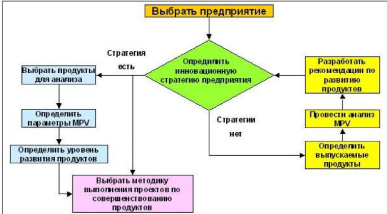
\includegraphics[width=.8\textwidth]{6.png}
\end{center}
Taken from the cited work of O. M. Gerasimov \cite{B9}.

"Step-by-step strategy" is often thought of as "easy TRIZ" and "step-by-step
algorithm" as "advanced TRIZ". This is not entirely true. For example,
G. Ivanov's ARIP \cite{B22} is a typical algorithm, although it is aimed at
easy perception by an untrained (in terms of TRIZ) listener.

It seems that the step-by-step strategy is more oriented towards mastery and
use by a specialist who remains an expert in his or her local field, simply
applying TRIZ as one of his or her working tools along with others.

The step-by-step algorithm requires considerably more, if not knowledge, then
skill TRIZ application and is used when a problem proves to be unsolved by
traditional methods. In practice, it is difficult to imagine a production
engineer being able to go through all the steps of ARIZ-91 in detail and
thoughtfully. TRIZ professionals also use this complicated tool only when
necessary. But on the other hand, when the problem is not solved head-on,
there is often nothing else to do.

Thus, both approaches look valid each in its own context. Therefore it seems
important to have two versions of the methodology for each TRIZ tool.

There is also a third approach for flow analysis. It has been repeatedly
mentioned above that flow analysis is a special special case of functional
analysis. Therefore, a special tool for organising such a transition is
desirable.

Therefore, this chapter provides three algorithms for different applications
of analysis.

\subsection{"Step-by-step algorithm" for conducting a flow analysis}

\begin{enumerate}
\item Select the system to be analysed, select the target gap. Draw up a
  component model for the flows and associated static components

  Note 1. As with FM, it is important to select components of the same system
  level, i.e. that are not components of each other. It is advisable to limit
  the number of components and threads to no more than 6-9.

  Note 2. It must be remembered that each material stream is always
  accompanied by auxiliary streams: the energy stream and the information
  stream. Excluding these auxiliary flows from consideration is possible, but
  it should always be a conscious choice. Particularly because the management
  of ancillary flows is often an important tool in the management of the main
  flow. Excluding them as early as the component model stage closes this
  possibility.

\item Make a model for the main flows (useful and harmful -- i.e. those
  defined by the principle of action).

  Note 3: The model is constructed as a graph in which the nodes are static
  model components and the links are flows, as shown in Appendix 2 of the
  Algorithm. The model takes into account:
  \begin{itemize}
  \item Availability of an additional time axis
  \item The need to separately identify useful and harmful flows and the
    area/time when a flow changes from a useful to a harmful one
  \item Availability of flow transformations
  \item the places where parasitic flows originate and exit into the
    supersystem
  \item the presence of closed streams
  \end{itemize}
\item If necessary, add energy and information flows to the model

  Note 4: The order in which the flows are introduced can be changed, e.g. if
  the project is "energy" or "information" in nature. But when different types
  of flows are considered in the model, this order is appropriate.

\item If necessary, add parasitic flows to the model.

  Note 5. Different types of flows are colour coded in the model column. In
  the table, the designation is in a separate column, although it is more
  convenient to duplicate the colour for clarity.

\item Determine the values of the main parameter of each of the streams and
  assess the level of that parameter on an Excessive/Adequate/Inadequate
  scale.

  Note 6: Most often (but not necessarily!) the main parameter for flow is its
  intensity ([A=K/s], [m3/s], etc.).

  It is often difficult to set absolute values for parameters. In this case
  you should at least specify a possible range.

\item Mark harmful and parasitic flows and inadequate flows on the graph with
  different colours

\item Due to the formality of the procedure in steps 2-4, there may be flows
  in the model that are not realistically flowing. Remove them from the model.

  Note 7. An important, but optional, feature of such a flow is the absence of
  parameter values as such.

\item Make a model in tabular form

  Note 8: A table and a graph can be made at the same time. But more often it
  is more convenient to make the graph first and then the table. The graph
  shows the structure of the flows, while the table shows their parameters

\item Given the chosen target weakness, remove insignificant (non-significant)
  flows. In the same step, remove those flow channels where the flow does not
  undergo any meaningful change
  
  Note 9. Flows of low absolute intensity as well as flows that are not
  significant within the scope of this project can be taken as insignificant.

  Note 10. During the analysis we do not yet know in advance which flow is
  important (otherwise no analysis is needed). Therefore it should be done
  very carefully. When in doubt, it is better to leave an unimportant flow in
  the model than to remove one which may later turn out to be the key flow. In
  case of serious doubts, step 8 can be skipped.

\item Remove channels from the model graph (without removing them from the
  table)

  Note 11. Flows undergo minor changes in the channel. Therefore they can be
  removed from the graph to simplify the visual perception. However, the
  channels must remain in the tabular form of the model!

  At the same time the correct channel definition is checked: if a component
  makes strong changes to a stream, it is more correct to classify it as the
  receiver of the stream (and at the same time the source of the next,
  transformed stream).

  Note 12. Points 8-10 are performed to simplify the model. In the case of a
  sufficiently simple and illustrative model, the following may be omitted

\item Refine the table form of the model according to the results of items 9,
  10, 11. 

  Note 12a. Points 9-12 are intended to simplify the model in case it proves
  to be overloaded with unnecessary components. For relatively simple models,
  the points can be omitted. In the FA, these points correspond to the
  recommendation of iterative procedures.

\item Identify sections of the flow model that have disadvantages. The
  disadvantages are:
  \begin{itemize}
  \item flow areas with inadequate parameters (including bottle necks and
    stagnant areas)
  \item areas where the channel changes (disrupts) the flow or the flow
    changes (disrupts) the channel
  \item grey areas
  \item high-loss flow conversion points
  \item points of occurrence of parasitic flows
  \end{itemize}
  The selection should be made by introducing additional columns in the
  tabular form of the model.

  Note 13. Flaws can also be highlighted on the graph. However, very often the
  graph becomes overloaded with different designations and difficult to
  perceive visually. Therefore, the analytical points of the algorithm need to
  be tabulated, putting only the information that is perceptible (based on the
  project objectives) into the graph.

\textbf{The analytical part of the algorithm}

\item Identify fragments with (and interacting with) homogeneous
  flows. Formulate (clarify) disadvantages.

\item Classify all harmful or inadequately performed beneficial flows by
  classification attributes (see Appendix 1 "Flow Classifier").

\item Write down a list of the shortcomings identified and rank them

  Note 14. When ranking, use the data from step 12. In addition, it may be
  necessary to construct a causal chain of deficiencies.

\item Formulate the flaw elimination objectives with respect to flow
  parameters or channel elements, taking into account the recommendations set
  out in Chapters 4-7 and Appendix 1 "typical methods for flaw elimination in
  a flow model".

\item The basic principles for remedying the shortcomings found.
  \begin{itemize}
  \item Deficiencies that do not form a contradiction are usually remedied by
    sectoral techniques and methods.
  \item Gaps that form conflicting requirements for flows and/or related
    components should be resolved first -- using the techniques and
    recommendations described in the chapter "flow classification"
  \item For deficiencies formulated in relation to channel parameters -- See
    chapter "Transition from flow analysis to functional analysis"
    
    Note 15. Basic (typical) channel properties that are relatively easy to
    change:
    \begin{itemize}
    \item Channel conductivity parameters
      \begin{itemize}
      \item Bottle neck
      \item Stagnant (buffer) zone
      \item Channel length
      \item Specific channel resistance
      \item Density of flow in the channel
      \item Number of flow conversions
      \end{itemize}
    \item Parameters for flow variation
      \begin{itemize}
      \item Grey area
      \item The channel changes (disrupts) the flow
      \item The flow changes (destroys) the channel.
      \end{itemize}
    \item For deficiencies formulated in relation to flow parameters --
      formulate problems for source/consumer pair. See appendix 1.
    \end{itemize}
  \end{itemize}
  Note 16. For example, if you want to increase the voltage in a transmission
  line -- start with the transformers and only post look at the line itself.
  If we want to increase the pressure in a gas pipeline -- look at the booster
  compressor and only then think about the pipe

  Note 17. See appendix 2 for an example of this algorithm. The streaming
  analysis shown in this appendix was performed during the execution of a real
  project for Samsung SDI. Due to confidentiality conditions, a number of
  numerical values have been omitted. In addition, some steps are not shown in
  full but as examples (Sanky diagrams, solution examples). This example is an
  example of a complex analysis, after unsuccessful attempts to perform a flow
  analysis using the traditional method.
\end{enumerate}

\subsection{Transition from flow analysis to functional analysis}

As already stated, flow analysis is a special case of functional analysis. It
is often necessary to consider the interaction of static components not only
with flows but also with each other. The procedure for changing from flow
analysis to functional analysis is described below.
\begin{enumerate}
\item Building PMs using the proposed methodology
\item Identification of flow deficiencies as recommended
\item Clarification of the deficiencies identified, identifying the type of
  deficiencies:
  \begin{itemize}
  \item Inadequate flow parameters and functions
  \item Inadequate and harmful flow functions,
  \item Excessive payback factor for the functioning of the stream
  \item Inadequate channel parameters and functions
  \item Inadequate and harmful channel functions
  \item Excessive payback factor for the formation and functioning of the
    canal
  \end{itemize}
\item Build a functional model for the components associated with the problem
  stream and conduct a standard FA.

  Note 18. In fact, this is a standard and widely used technique by
  practitioners: construct a detailed deeper system level FM for the
  problematic part of the system identified by the higher level models.

\item Formulate the disadvantages associated with the interaction of static
  components, formulate tasks to eliminate them.
\end{enumerate}

\subsection{A "step-by-step strategy" for conducting a flow analysis}

In comparatively simple cases this may be sufficient. Recommended for
specialists in specific fields.
\begin{enumerate}
\item Identify streams.

  Write out the existing flows in the system that are relevant to the project
  objective

\item Specify the type of flow: useful/harmful/parasitic.

For useful flows, specify the level of fulfilment of the main function:
adequate/insufficient/abundant

\item For each stream, define source, channel, receiver.

\item Classify the flows.

  To classify according to chapter 3 "Flow types"

\item Articulate the disadvantages.

  Accept harmful and parasitic flows as disadvantages, as well as inadequate
  performance of the main function by the useful flow

\item Formulate objectives to address the shortcomings.
\end{enumerate}

\begin{thebibliography}{xxx}
\bibitem{B1} Altshuller G.S. \foreignlanguage{russian}{Творчество как точная
  наука} -- Creativity as an exact science. Moscow: Sov. Radio, 1979.

\bibitem{B2} Altshuller G.S., Zlotin B.L., Zusman A.V. et al.
  \foreignlanguage{russian}{Поиск новых идей: от озарения к технологии (теория
    и практика решения изобретательских задач)} -- Search for New Ideas: From
  Insight to Technology (Theory and Practice of Inventive Problem Solving).
  Kishinev, "Cartea Moldoveiasca", 1989.
  \url{http://www.trizway.com/content/poisk_novih1.pdf}

\bibitem{B3} Salamatov Y.A., 1991-1996. \foreignlanguage{russian}{Система
  Законов Развития Техники (Основы Теории Развития Технических Систем)} --
  System of Technological Development Laws (Fundamentals of Technical Systems
  Development Theory).  \url{http://www.trizminsk.org/e/21101440.htm}

  Salamatov, Y.A. TRIZ: the Right Solution at the Right Time: a Guide to
  Innovative Problem Solving.

\bibitem{B4} \foreignlanguage{russian}{Энергетический анализ технических
  систем} -- Energy Analysis of Technical Systems. Baku, 1974.

\bibitem{B5} Petrov V.M. \foreignlanguage{russian}{Законы развития систем} --
  The Laws of Systems Development. A Series of texts, 24 September 2002.
  \url{http://www.trizland.ru/trizba/pdf-books/zrts-12-microlevel.pdf}
  \url{http://www.trizland.ru/trizba/pdf-books/zrts-16-energo.pdf}

\bibitem{B6} Litvin S.S., Lyubomirsky A.L. \foreignlanguage{russian}{Законы
  развития технических систем} -- Laws of development of technical systems.
  February 2003. \url{http://www.metodolog.ru/00822/00822.html}

\bibitem{B7} Gerasimov V.M. et al. \foreignlanguage{russian}{Применение
  методов технического творчества при проведении функционально-стоимостного
  анализа: Методические рекомендации} -- Application of Technical Creativity
  Methods in Functional Value Analysis: Methodological Recommendations. Moscow:
  "Informelektro", 1990.

\bibitem{B8} Gerasimov V.M. et al. \foreignlanguage{russian}{Основные
  положения методики проведения функционально-стоимостного анализа:
  Методические рекомендации} -- Main Provisions of the Methodology of
  Functional Value Analysis: Methodological Recommendations, Moscow:
  Inform-FSA, 1991.

\bibitem{B9} Gerasimov O.M. \foreignlanguage{russian}{Технология выбора
  инструментов инновационного проектирования на основе ТРИЗ-ФСА} -- Technology
  of Innovative Design Tools Selection Based on TRIZ-FVA.
  \url{http://triz-summit.ru/ru/203864/204737/204739}
  
\bibitem{B10} Efimov A.V. \foreignlanguage{russian}{Потоковый анализ
  технологических операций} -- Flow analysis of technological operations.
  \url{http://www.metodolog.ru/01463/01463.html}
  
\bibitem{B11} Kashkarov A.G.
  \foreignlanguage{russian}{Вещественно-энергетические преобразования в
    технической системе. Методика построения и анализа моделей.} -- Material
  and energy transformations in a technical system. Methodology of Model
  Construction and Analysis.
  \url{http://triz-summit.ru/ru/203864/204357/204590/}

\bibitem{B12} \url{http://infographer.ru/sankey-diagrams/}

\bibitem{B13} Energy and the challenge of sustainability 

\bibitem{B14} \foreignlanguage{russian}{АРИЗ-91 МУНТТР, Часть 2} -- ARIZ-91,
  Part 2.  \url{http://triz-summit.ru/205253/203840/204230/204231/204295/}

\bibitem{B16} Gerasimov O.M. \foreignlanguage{russian}{Технология выбора
  инструментов инновационного проектирования на основе ТРИЗ-ФСА} -- Technology
  for selecting innovation design tools based on TRIZ and FVA.
  \url{http://triz-summit.ru/ru/203864/204737/204739/}
  
\bibitem{B18} \foreignlanguage{russian}{Защита автомобильных дорог от селевых
  потоков.  Информационный сборник.} -- Road protection from sluge and mud
  flows. Information collection.
  \url{http://www.znaytovar.ru/gost/2/Avtomobilnye_dorogi_Nauchnotex.html}

\bibitem{B19} Mitsubishi Pajero iO Mezurashī kemono.
  \foreignlanguage{russian}{Бортжурнал. Немного о картерных газах.} --
  Logbook.  A little bit about crankcase gases.
  \url{http://www.drive2.ru/l/670559/}

\bibitem{B20} Lenyashin V.A., Hyo-jun Kim -- \foreignlanguage{russian}{Вредная
  система.  Использование этого понятия в современной ТРИЗ} -- Harmful system.
  The use of this concept in modern TRIZ.
  \url{http://www.metodolog.ru/00859/00859.html}
  
\bibitem{B21} ARIZ-68 \url{http://www.altshuller.ru/triz/ariz68.asp}

\bibitem{B22} ARIP-2011 \url{http://www.trizland.ru/trizba/1886}
\end{thebibliography}

\end{document}
